% ======================================================================
%  FYS4480/FYS9480  Quantum mechanics for many-particle systems
%  Week 45, November 5-6, 2026
%  Lecture slides (Beamer).  Thursday: 2 x 45 min,  Friday: 2 x 45 min.
%
%  Sources: chapter9.tex, section "Diagrammatic approach and the linked
%  diagram theorem" (9.15): the perturbation drawn, first and second order,
%  "Where the rules come from" (the four rules derived from Wick's theorem),
%  "Third order" (fourteen diagrams, MP3, the pairing model diagram by
%  diagram) and "Unlinked diagrams and the linked-diagram theorem".
%  Thursday opens with the week-44 lecture 4 that was not delivered (every
%  contribution to the energy through fourth order and to the wave operator
%  through third order).  Week 46: the proof of the linked-diagram theorem.
%  Answers to the week-44 exercises (Exercises/AnswersWeek44.tex) and the
%  week-45 exercises (Exercises/ExercisesWeek45.tex) are on the last frames.
%  Companion program: BookPrograms/chapter09/diagrams.py; notebook week45.ipynb.
%  Diagram styles (pline, hline, vint, vtx, fvtx, hloop, fcidiagram) are
%  those of book.tex, so the chapter's TikZ figures compile unchanged.
%
%  Build:  pdflatex week45.tex  (twice)
% ======================================================================
\documentclass[aspectratio=169,10pt]{beamer}

% ---------------------------------------------------------------- packages
\usepackage[utf8]{inputenc}
\usepackage[T1]{fontenc}
\usepackage{amsmath,amssymb,bm,mathtools}
\usepackage{booktabs}
\usepackage[most]{tcolorbox}
\usepackage{listings}
\usepackage{hyperref}
\usepackage{tikz}
\usetikzlibrary{positioning,arrows.meta,decorations.markings,shapes.misc}
\usetikzlibrary{tikzmark}

% ---------------------------------------------------------------- look
\usetheme{default}
\useinnertheme{rectangles}
\setbeamertemplate{navigation symbols}{}
\definecolor{uioblue}{RGB}{18,52,86}
\definecolor{teal}{RGB}{0,128,128}
\definecolor{warm}{RGB}{181,73,36}
\definecolor{paleblue}{RGB}{232,240,248}
\definecolor{paleteal}{RGB}{228,244,244}
\definecolor{palewarm}{RGB}{252,238,230}
\definecolor{palegreen}{RGB}{232,244,234}
\setbeamercolor{structure}{fg=uioblue}
\setbeamercolor{title}{fg=uioblue}
\setbeamercolor{frametitle}{fg=uioblue,bg=white}
\setbeamercolor{section in toc}{fg=uioblue}
\setbeamercolor{alerted text}{fg=warm}
\setbeamercolor{block title}{fg=white,bg=uioblue}
\setbeamercolor{block body}{bg=paleblue}
\setbeamercolor{block title example}{fg=white,bg=teal}
\setbeamercolor{block body example}{bg=paleteal}
\setbeamerfont{frametitle}{size=\large,series=\bfseries}
\setbeamerfont{title}{size=\LARGE,series=\bfseries}
\setbeamertemplate{frametitle}{%
  \vspace*{0.6em}\insertframetitle\par
  \vspace*{-0.2em}{\color{teal}\rule{\textwidth}{0.6pt}}}
\setbeamertemplate{footline}{%
  \hbox{\begin{beamercolorbox}[wd=\paperwidth,ht=2.4ex,dp=1.2ex,leftskip=1em,rightskip=1em]{structure}%
  \footnotesize FYS4480/9480 -- Week 45 \hfill \insertsection \hfill \insertframenumber/\inserttotalframenumber
  \end{beamercolorbox}}}
\setbeamertemplate{itemize items}[circle]
\setbeamertemplate{enumerate items}[default]
\setbeamertemplate{section page}{%
  \begin{centering}
    {\usebeamerfont{section title}\usebeamercolor[fg]{title}\LARGE\bfseries\insertsection\par}
    \vspace{0.5em}{\color{teal}\rule{0.5\textwidth}{1pt}}
  \end{centering}}
\AtBeginSection[]{\frame{\sectionpage}}

% ---------------------------------------------------------------- boxes
\newcounter{thinkctr}
\newcommand{\thinkq}[2]{%
  \stepcounter{thinkctr}%
  \vfill
  \begin{tcolorbox}[enhanced,colback=palewarm,colframe=warm,boxrule=1.2pt,arc=4pt,
    grow to left by=6mm,grow to right by=6mm,
    left=16pt,right=16pt,top=16pt,bottom=18pt,
    fonttitle=\bfseries\Large,fontupper=\Large,
    title={Pause to think \#\thethinkctr\hfill\mdseries\normalsize(about #1 min -- discuss with your neighbour)}]
  #2
  \end{tcolorbox}
  \vfill}
\newcommand{\thinka}[1]{%
  \vfill
  \begin{tcolorbox}[enhanced,colback=paleteal,colframe=teal,boxrule=1.2pt,arc=4pt,
    grow to left by=6mm,grow to right by=6mm,
    left=16pt,right=16pt,top=16pt,bottom=18pt,
    fonttitle=\bfseries\Large,fontupper=\large,
    title={Answer to pause \#\thethinkctr}]
  #1
  \end{tcolorbox}
  \vfill}
\newcommand{\mbbox}[1]{%
  \begin{tcolorbox}[colback=paleblue,colframe=uioblue,title={\bfseries Many-body connection}]
  #1
  \end{tcolorbox}}
\newcommand{\warnbox}[1]{%
  \begin{tcolorbox}[colback=palewarm,colframe=warm,title={\bfseries A trap to avoid}]
  #1
  \end{tcolorbox}}
\newcommand{\numbox}[1]{%
  \begin{tcolorbox}[colback=palegreen,colframe=teal!70!black,title={\bfseries Measured}]
  #1
  \end{tcolorbox}}

% ---------------------------------------------------------------- code
\lstset{language=Python,basicstyle=\ttfamily\scriptsize,
  keywordstyle=\color{uioblue}\bfseries,commentstyle=\color{teal},
  stringstyle=\color{warm},showstringspaces=false,columns=fullflexible,
  frame=single,rulecolor=\color{paleblue},backgroundcolor=\color{white},
  breaklines=true}

% ---------------------------------------------------------------- macros
\newcommand{\ket}[1]{\vert #1\rangle}
\newcommand{\bra}[1]{\langle #1\vert}
\newcommand{\braket}[2]{\langle #1\vert #2\rangle}
\newcommand{\element}[3]{\langle #1\vert #2\vert #3\rangle}
\DeclareMathOperator{\tr}{tr}
\newcommand{\bigO}{\mathcal{O}}
\newcommand{\bmat}[1]{\bm{#1}}
\newcommand{\Amat}[1]{\bm{A}^{#1}}
\newcommand{\Bmat}[1]{\bm{B}^{#1}}
\newcommand{\hH}{\hat{H}}
\newcommand{\ad}[1]{a_{#1}^{\dagger}}
\newcommand{\ketbra}[2]{\vert #1\rangle\langle #2\vert}
% normal ordering with respect to the reference determinant |c> (as in week 40)
\newcommand{\nc}[1]{\bigl\{#1\bigr\}}

% ---------------------------------------------------------------- diagrams
\tikzset{
  tens/.style={draw=uioblue,fill=paleblue,thick,rounded corners=1pt,minimum size=7mm,font=\small},
  mpo/.style={draw=warm,fill=palewarm,thick,rounded corners=1pt,minimum size=7mm,font=\small},
  env/.style={draw=teal!70!black,fill=paleteal,thick,rounded corners=1pt,
              minimum width=7mm,minimum height=14mm,font=\small},
  leg/.style={thick,uioblue},
  dlab/.style={font=\scriptsize},
  every picture/.style={scale=0.8,baseline=(current bounding box.center)}
}

\graphicspath{{../BookFigures/}{./}}

\newcommand{\dd}{\mathrm{d}}


% ---------------------------------------------------------------- MBPT macros
\newcommand{\mel}[3]{\langle #1\lvert #2\rvert #3\rangle}
\newcommand{\av}[1]{\langle #1\rangle_0}
\newcommand{\cre}[1]{a_{#1}^{\dagger}}
\newcommand{\ann}[1]{a_{#1}}
\newcommand{\no}[1]{\bigl\{#1\bigr\}}
\newcommand{\vbar}[4]{\overline v_{#1#2#3#4}}
\newcommand{\Eref}{E_{\mathrm{ref}}}
\newcommand{\ph}{\Phi_0}
\newcommand{\Psizero}{\Psi_0}
\newcommand{\ord}[1]{\mathcal O(#1)}
\newcommand{\Rzero}{R_0}
\tikzset{fermion/.style={line width=.8pt,uioblue,postaction={decorate},decoration={markings,mark=at position .56 with {\arrow{Stealth}}}},
  interaction/.style={dashed,line width=.8pt,warm},
  vertex/.style={circle,fill=warm,inner sep=1.7pt}}
% ---- the Goldstone-diagram styles of book.tex (chapter 5, 9 figures)
\tikzset{
  pline/.style={thick,uioblue,postaction={decorate},
    decoration={markings,mark=at position 0.55 with {\arrow{Stealth[length=5pt]}}}},
  hline/.style={thick,uioblue,postaction={decorate},
    decoration={markings,mark=at position 0.55 with {\arrowreversed{Stealth[length=5pt]}}}},
  vint/.style={dashed,thick,warm},
  vtx/.style={circle,fill=warm,inner sep=1.4pt},
  fvtx/.style={cross out,draw=warm,thick,minimum size=5pt,inner sep=0pt},
  dlab/.style={font=\scriptsize},
  hloop/.style={thick,uioblue,postaction={decorate},
    decoration={markings,mark=at position 0.5 with {\arrow{Stealth[length=5pt]}}}},
  fcidiagram/.style={scale=0.9,baseline=(current bounding box.center)}}
\newcommand{\ftil}[1]{\tilde f_{#1}}
\newcommand{\W}{W}
\newcommand{\wickpattern}[1]{%
\begin{tikzpicture}[x=.86cm,y=.72cm,every node/.style={font=\small,inner sep=1.3pt},scale=1,baseline=(current bounding box.center)]
\node(p)at(0,0){\(\cre{p}\)};\node(q)at(1,0){\(\cre{q}\)};
\node(s)at(2,0){\(\ann{s}\)};\node(r)at(3,0){\(\ann{r}\)};
\node(a)at(4,0){\(\cre{a}\)};\node(b)at(5,0){\(\cre{b}\)};
\node(j)at(6,0){\(\ann{j}\)};\node(i)at(7,0){\(\ann{i}\)};
\draw[uioblue,line width=.6pt,rounded corners=3pt](p.north)--++(0,1.05)-|(i.north);
\draw[uioblue,line width=.6pt,rounded corners=3pt](q.north)--++(0,.64)-|(j.north);
\ifnum#1=1\relax
\draw[teal,line width=.7pt,rounded corners=3pt](s.south)--++(0,-.9)-|(b.south);
\draw[teal,line width=.7pt,rounded corners=3pt](r.south)--++(0,-.48)-|(a.south);
\else
\draw[teal,line width=.7pt,rounded corners=3pt](s.south)--++(0,-.9)-|(a.south);
\draw[teal,line width=.7pt,rounded corners=3pt](r.south)--++(0,-.48)-|(b.south);
\fi
\end{tikzpicture}}


% ---------------------------------------------------------------- title
\title{Many-body perturbation theory: diagram rules, third order and the linked-diagram theorem}
\subtitle{FYS4480/FYS9480 -- Week 45, November 5--6, 2026}
\author{Cecilie Glittum and Morten Hjorth-Jensen}
\institute{Department of Physics,\\
University of Oslo, Norway}
\date{}

\begin{document}

\begin{frame}[plain]
  \vspace*{-0.2em}{\setbeamerfont{title}{size=\Large,series=\bfseries}\titlepage}
  \vfill
  \begin{center}\small
  Thursday: every contribution to the energy through fourth order and to the wave operator through third (the list from week 44), then the diagrams: contractions are lines, cuts are denominators, and the four rules -- sums, denominators, $\tfrac12$ per pair of equivalent lines, $(-1)^{h+l}$ -- derived from Wick's theorem\\
  Friday: the fourteen third-order diagrams, MP3 and the pairing model diagram by diagram; unlinked diagrams at fourth order, the factorisation of denominators, and the linked-diagram theorem\\[0.8em]
  {\footnotesize Reading: lecture notes chapter 9, section 9.15 (diagrammatic approach and the linked diagram theorem); Shavitt and Bartlett, chapters 4--5. Code: \texttt{BookPrograms/chapter09/diagrams.py}; notebook \texttt{week45.ipynb}.\\[0.2em]
  Answers to the week-44 exercises and the week-45 exercises: last frames.}
  \end{center}
\end{frame}

\begin{frame}[shrink=12]{Plan for week 45}
  \begin{block}{Thursday, $2\times45$ min: the lists, and the rules derived}
    \begin{itemize}
      \item From week 44: the recursion, $\Omega^{(1,2,3)}$ and $E^{(1,2,3,4)}$ in resolvent form and in the determinant basis
      \item Normal ordering the vertices, $H_I=E^{(1)}+W$, absorbs every renormalisation term with a factor $E^{(1)}$: $E^{(3)}=\av{WR_0WR_0W}$
      \item Contractions are lines; cuts are denominators ($[H_0,\cre{p}]=\varepsilon_p\cre{p}$); what $Q$ removes
      \item The weight ($4^{n_V}$ relabellings, equivalent lines) and the sign (vertex ends, the permutation $\pi$, $(-1)^{K-l}(-1)^p=(-1)^{h+l}$)
      \item First and second order re-read with the rules
    \end{itemize}
  \end{block}
  \begin{block}{Friday, $2\times45$ min: third order and the linked-diagram theorem}
    \begin{itemize}
      \item Third order by intermediate states: fourteen connected diagrams, three of them MP3 (pp ladder, hh ladder, ph ring); the pairing model diagram by diagram, $-\tfrac{53}{576}-\tfrac{53}{576}+\tfrac{29}{288}=-\tfrac1{12}$ (units of $g^3$)
      \item Fourth order: the unlinked diagrams, the factorisation of their denominators, and the folded term $-E^{(2)}\av{WR_0^2W}$ that removes them
      \item \alert{The linked-diagram theorem}: energy = connected closed diagrams, wave operator = linked diagrams; extensivity, Brillouin-Wigner, partial summations. The proof: week 46
    \end{itemize}
  \end{block}
\end{frame}

\begin{frame}[shrink=12]{Where we are, and the route through this week}
  \begin{columns}[T]
    \column{0.5\textwidth}
    \begin{block}{Done}
      \begin{itemize}
        \item Full CI (weeks 37--38): exact, exponential; the amplitude equations drawn as diagrams with four rules we did not prove
        \item Hartree-Fock (weeks 38--39): $f_{ai}=0$
        \item Week 44: $P$, $Q$, the resolvent, BW versus RS, $E^{(2)}$ from Wick's theorem, a two-level benchmark
      \end{itemize}
    \end{block}
    \column{0.5\textwidth}
    \begin{block}{This week}
      \begin{enumerate}
        \item The complete lists through fourth order
        \item The four rules, with proofs
        \item Third order: fourteen diagrams
        \item Unlinked diagrams and the theorem
      \end{enumerate}
    \end{block}
  \end{columns}
  \vspace{0.6em}
  \mbbox{Notation as in week 44: $H=H_0+H_I$ with $H_0=\sum_p\varepsilon_p\cre{p}\ann{p}$, reference $\ket{\ph}$ with $\varepsilon_0=\sum_{i}\varepsilon_i$, $R_0=Q/(\varepsilon_0-H_0)$, $D_m=\varepsilon_0-\varepsilon_m$, $\av{X}=\mel{\ph}{X}{\ph}$, $V_{mn}=\mel{\Phi_m}{H_I}{\Phi_n}$. Occupied $i,j,k,l$, empty $a,b,c,d$. Antisymmetrised elements $\vbar{p}{q}{r}{s}=\langle pq|v|rs\rangle_{\rm AS}$ throughout.}
\end{frame}

% ======================================================================
\section{Thursday, lecture 1: The lists, and from sums to pictures}
% ======================================================================

\begin{frame}{The recursion that generates every order (week 44, lecture 4)}
With \(R_0=Q/(\varepsilon_0-H_0)\) and \(\ket{\Psizero}=\sum_n\ket{\Psi^{(n)}}\), \(\ket{\Psi^{(0)}}=\ket{\ph}\), collecting powers of \(\eta\) in \(\ket{\Psizero}=\ket{\ph}+R_0(H_I-\Delta E)\ket{\Psizero}\) gives
\[
\boxed{\ket{\Psi^{(n)}}=R_0\Bigl[H_I\ket{\Psi^{(n-1)}}-\sum_{k=1}^{n-1}E^{(k)}\ket{\Psi^{(n-k)}}\Bigr],
\qquad
E^{(n+1)}=\mel{\ph}{H_I}{\Psi^{(n)}}.}
\]
\begin{itemize}
\item The subtracted terms are the normalisation (``renormalisation'', ``unlinked'') corrections; they appear from \(n=2\) on.
\item \(R_0\ket{\ph}=0\): every \(\ket{\Psi^{(n)}}\), \(n\ge1\), lies in \(Q\) space, so intermediate normalisation is preserved order by order.
\item \texttt{mbpt.py} implements exactly this recursion and checks it against the explicit expressions on the next two frames.
\end{itemize}
\end{frame}

\begin{frame}[shrink=5]{All contributions to the wave operator through third order}
Write \(\ket{\Psizero}=\Omega\ket{\ph}\) with \(\Omega=1+\Omega^{(1)}+\Omega^{(2)}+\Omega^{(3)}+\cdots\), \(R\equiv R_0\), \(V\equiv H_I\):
\begin{align*}
\Omega^{(1)}&=RV,\\[2pt]
\Omega^{(2)}&=RVRV\;-\;E^{(1)}R^2V,\\[2pt]
\Omega^{(3)}&=RVRVRV\;-\;E^{(1)}\bigl[RVR^2V+R^2VRV\bigr]\;+\;\bigl(E^{(1)}\bigr)^2R^3V\;-\;E^{(2)}R^2V .
\end{align*}
In the determinant basis, with \(V_{mn}=\mel{\Phi_m}{H_I}{\Phi_n}\) and \(D_m=\varepsilon_0-\varepsilon_m\) (\(m,n,l\ne0\)):
\begin{align*}
\langle\Phi_m|\Psi^{(1)}\rangle&=\frac{V_{m0}}{D_m},\qquad
\langle\Phi_m|\Psi^{(2)}\rangle=\sum_{n}\frac{V_{mn}V_{n0}}{D_mD_n}-\frac{V_{00}V_{m0}}{D_m^2},\\
\langle\Phi_m|\Psi^{(3)}\rangle&=\sum_{nl}\frac{V_{mn}V_{nl}V_{l0}}{D_mD_nD_l}
-V_{00}\Bigl[\sum_n\frac{V_{mn}V_{n0}}{D_mD_n^2}+\sum_n\frac{V_{mn}V_{n0}}{D_m^2D_n}\Bigr]
+V_{00}^2\frac{V_{m0}}{D_m^3}
-E^{(2)}\frac{V_{m0}}{D_m^2}.
\end{align*}
\small For a two-body \(H_I\): \(\Psi^{(1)}\) has singles (\(U_{ai}/(\varepsilon_i-\varepsilon_a)\)) and doubles (\(\vbar{a}{b}{i}{j}/(\varepsilon_i+\varepsilon_j-\varepsilon_a-\varepsilon_b)\)); \(\Psi^{(2)}\) reaches up to quadruples; \(\Psi^{(3)}\) up to sextuples. Rank is not order.
\end{frame}

\begin{frame}[shrink=5]{All contributions to the energy through fourth order}
With \(\av{X}=\mel{\ph}{X}{\ph}\), \(R=Q/(\varepsilon_0-H_0)\), \(V=H_I\), and \(E^{(n+1)}=\av{V\Omega^{(n)}}\):
\begin{align*}
E^{(1)}&=\av{V},\\[2pt]
E^{(2)}&=\av{VRV},\\[2pt]
E^{(3)}&=\av{VRVRV}\;-\;E^{(1)}\av{VR^2V},\\[2pt]
E^{(4)}&=\av{VRVRVRV}\;-\;E^{(1)}\bigl[\av{VR^2VRV}+\av{VRVR^2V}\bigr]\;+\;\bigl(E^{(1)}\bigr)^2\av{VR^3V}\;-\;E^{(2)}\av{VR^2V}.
\end{align*}
In the determinant basis:
\begin{align*}
E^{(1)}&=V_{00},\qquad E^{(2)}=\sum_m\frac{V_{0m}V_{m0}}{D_m},\qquad
E^{(3)}=\sum_{mn}\frac{V_{0m}V_{mn}V_{n0}}{D_mD_n}-V_{00}\sum_m\frac{V_{0m}V_{m0}}{D_m^2},\\
E^{(4)}&=\sum_{mnl}\frac{V_{0m}V_{mn}V_{nl}V_{l0}}{D_mD_nD_l}
-2V_{00}\sum_{mn}\frac{V_{0m}V_{mn}V_{n0}}{D_m^2D_n}
+V_{00}^2\sum_m\frac{V_{0m}V_{m0}}{D_m^3}
-\Bigl(\sum_n\frac{V_{0n}V_{n0}}{D_n}\Bigr)\sum_m\frac{V_{0m}V_{m0}}{D_m^2}.
\end{align*}
\small (The two mixed terms are complex conjugates, equal for real matrix elements, hence the \(2\).) Every term with a factor \(E^{(k)}\) in front is a renormalisation term: the product of two separately evaluated pieces. Today: these are the \emph{unlinked} diagrams, and they cancel against the unlinked parts of the principal term -- the linked-diagram theorem.
\end{frame}

\begin{frame}[shrink=8]{The same list in the language of determinants, through second order}
For \(H_0=\sum_p\varepsilon_p\cre{p}\ann{p}\) and \(H_I=E^{(1)}+U_N+V_N\):
\begin{align*}
E^{(1)}&=\sum_{i}u_{ii}+\frac12\sum_{ij\in\mathrm{occ}}\vbar{i}{j}{i}{j}
\quad(\text{with } u=0 \text{ for a diagonal } h_0),\\[2pt]
E^{(2)}&=\underbrace{\sum_{ia}\frac{|U_{ai}|^2}{\varepsilon_i-\varepsilon_a}}_{1p1h}
+\underbrace{\frac14\sum_{ijab}\frac{|\vbar{a}{b}{i}{j}|^2}{\varepsilon_i+\varepsilon_j-\varepsilon_a-\varepsilon_b}}_{2p2h},\\[2pt]
\Omega^{(1)}\ket{\ph}&=\sum_{ia}\frac{U_{ai}}{\varepsilon_i-\varepsilon_a}\ket{\Phi_i^a}
+\frac14\sum_{ijab}\frac{\vbar{a}{b}{i}{j}}{\varepsilon_i+\varepsilon_j-\varepsilon_a-\varepsilon_b}\ket{\Phi_{ij}^{ab}}.
\end{align*}
\numbox{Four models, \texttt{mbpt.py}: the fourth order from the explicit formula and from the recursion agree to \(10^{-12}\). Hubbard (\(U=2\)): the four pieces are \(-0.191\), \(+0.303\), \(-0.151\), \(+0.032\) and the total \(-0.0076\). Pairing (\(g=0.5\)): \(E^{(3)}\) is \(-0.02300347-(-0.01258681)=-0.01041667\). The cancellations are severe, and they are the point of this week.}
\end{frame}

\begin{frame}{Pause to think \#1}
\thinkq{3}{Look at the list of fourth-order terms.
\begin{enumerate}
\item How many distinct terms does \(E^{(4)}\) have for a reference with \(E^{(1)}=0\) (Hartree-Fock partition with the mean field in \(H_0\))?
\item In the third order, \(E^{(1)}\av{VR^2V}\) is the product of two quantities that are each sums over the whole system. If the system were two non-interacting copies of a smaller one, how would this product scale with the number of copies? And \(E^{(3)}\) itself?
\end{enumerate}}
\end{frame}

\begin{frame}{Answer to pause \#1}
\thinka{%
\begin{enumerate}
\item Two: the principal term \(\av{VRVRVRV}\) and the folded term \(-E^{(2)}\av{VR^2V}\). For the Lipkin model (\(E^{(1)}=0\)) \texttt{mbpt.py} gives \(-0.0036\) and \(+0.0072\), total \(+0.0036\).
\item \(E^{(1)}\) and \(\av{VR^2V}\) each scale linearly with the number of copies, so their product scales \emph{quadratically} -- an energy cannot. The principal term \(\av{VRVRV}\) contains a quadratically scaling piece of its own, and the subtraction removes it exactly: \(E^{(3)}\) scales linearly. This is size extensivity, verified to machine precision in chapter 9, and on Friday it becomes the statement that only \emph{linked} diagrams contribute.
\end{enumerate}}
\end{frame}

\begin{frame}[shrink=5]{Step zero: normal ordering absorbs the \(E^{(1)}\) renormalisation terms}
Write the perturbation in the normal-ordered form of week 44 (section 9.8), with a name for its non-scalar part:
\[
H_I=E^{(1)}+W,\qquad
\boxed{W=\sum_{pq}\ftil{pq}\no{\cre{p}\ann{q}}+\frac14\sum_{pqrs}\vbar{p}{q}{r}{s}\no{\cre{p}\cre{q}\ann{s}\ann{r}},}
\qquad
\ftil{pq}=u_{pq}+U_{pq}=f_{pq}-\varepsilon_p\delta_{pq},
\]
where \(f\) is the Fock matrix of week 39 and \(U_{pq}=\sum_{j}\vbar{p}{j}{q}{j}\) the mean field of the reference. \(\av{W}=0\), and every normal-ordered product has a vanishing reference expectation value.
\begin{block}{Look at the recursion}
The \(k=1\) term subtracts \(E^{(1)}\ket{\Psi^{(n-1)}}\) from \(H_I\ket{\Psi^{(n-1)}}\); the two combine into \(W\ket{\Psi^{(n-1)}}\). Since \(\braket{\ph}{\Psi^{(n)}}=0\) for \(n\ge1\), the energy formula may use \(W\) too:
\[
\boxed{\ket{\Psi^{(n)}}=R_0\Bigl[W\ket{\Psi^{(n-1)}}-\sum_{k=2}^{n-1}E^{(k)}\ket{\Psi^{(n-k)}}\Bigr],\qquad E^{(n+1)}=\mel{\ph}{W}{\Psi^{(n)}}\quad(n\ge1).}
\]
\end{block}
\(E^{(1)}\) has disappeared from the recursion, and with it \emph{every} renormalisation term carrying a factor \(E^{(1)}\).
\end{frame}

\begin{frame}[shrink=10]{The orders with normal-ordered vertices}
\[
\boxed{E^{(2)}=\av{WR_0W},\qquad
E^{(3)}=\av{WR_0WR_0W},\qquad
E^{(4)}=\av{WR_0WR_0WR_0W}-E^{(2)}\av{WR_0^2W}.}
\]
Third order: \emph{nothing to subtract}. Fourth order: only the folded term is left.
\begin{block}{The identity behind it is one line}
In the determinant basis \(W_{mn}=V_{mn}-V_{00}\delta_{mn}\), so
\[
\sum_{m,n\ne0}\frac{V_{0m}W_{mn}V_{n0}}{D_mD_n}
=\sum_{m,n\ne0}\frac{V_{0m}V_{mn}V_{n0}}{D_mD_n}-V_{00}\sum_{m\ne0}\frac{V_{0m}V_{m0}}{D_m^2}:
\]
the renormalisation term of third order \emph{is} the scalar part of the middle vertex, removed by not putting it there.
\end{block}
\numbox{Pairing model, \(g=0.5\): \(\av{WR_0WR_0W}=-0.01041667\), the whole third-order energy in one term. From here on every vertex is normal ordered: a cross carries \(\ftil{pq}\) (cross plus bubble of week 44), an interaction the antisymmetrised element.}
\end{frame}

\begin{frame}{The elements of a diagram (week 38, chapter 5)}
\begin{center}
\begin{tabular}{@{}c@{\hspace{2.5em}}c@{\hspace{2.5em}}c@{\hspace{2.5em}}c@{}}
  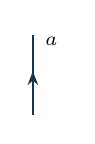
\begin{tikzpicture}[fcidiagram]
    \draw[pline] (0,0) -- (0,1.4); \node[dlab,right] at (0.05,1.3) {$a$};
  \end{tikzpicture} &
  \begin{tikzpicture}[fcidiagram]
    \draw[hline] (0,0) -- (0,1.4); \node[dlab,right] at (0.05,1.3) {$i$};
  \end{tikzpicture} &
  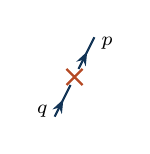
\begin{tikzpicture}[fcidiagram]
    \node[fvtx] (f) at (0,0.7) {}; \draw[pline] (-0.35,0) -- (f); \draw[pline] (f) -- (0.35,1.4);
    \node[dlab,right] at (0.3,1.3) {$p$}; \node[dlab,left] at (-0.3,0.1) {$q$};
  \end{tikzpicture} &
  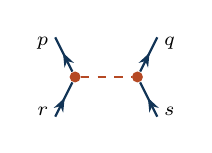
\begin{tikzpicture}[fcidiagram]
    \node[vtx] (v1) at (0,0.7) {}; \node[vtx] (v2) at (1.1,0.7) {}; \draw[vint] (v1) -- (v2);
    \draw[pline] (-0.35,0) -- (v1); \draw[pline] (v1) -- (-0.35,1.4);
    \draw[pline] (1.45,0) -- (v2); \draw[pline] (v2) -- (1.45,1.4);
    \node[dlab,left] at (-0.3,1.3) {$p$}; \node[dlab,left] at (-0.3,0.1) {$r$};
    \node[dlab,right] at (1.4,1.3) {$q$}; \node[dlab,right] at (1.4,0.1) {$s$};
  \end{tikzpicture}\\[0.3em]
  particle line & hole line & $\ftil{pq}$ (out $p$, in $q$) & $\vbar{p}{q}{r}{s}$: ends $(p,r)$ and $(q,s)$
\end{tabular}
\end{center}
\begin{itemize}
\item Time runs upward; the reference \(\ket{\ph}\) is the vacuum and is not drawn. Particle line: arrow up; hole line: arrow down.
\item Every vertex is a product of \emph{ends}, an end being \(\cre{\rm out}\ann{\rm in}\): the cross is one end, the interaction two ends joined by the dashed line, with the pairing \((p,r)\), \((q,s)\) of the matrix element.
\item New this week: between successive vertices sits \(R_0\); a horizontal \emph{cut} between them will give the denominator.
\end{itemize}
\small The four rules of week 38 (sums, denominators, \(\tfrac12\) per pair of equivalent lines, \((-1)^{h+l}\)) were stated and checked, not proved. Today they are proved.
\end{frame}

\begin{frame}[shrink=12]{A term of order \(n\) is a string, read from the bottom}
\[
\av{WR_0WR_0\cdots R_0W}=\mel{\ph}{W_nR_0W_{n-1}R_0\cdots R_0W_1}{\ph},
\]
the subscript numbering the vertices from the one that acts first (rightmost, bottom) to the one that acts last (leftmost, top).
\begin{block}{Forget the resolvents for a moment}
Each \(W_k\) is a sum of normal-ordered monomials. The generalised Wick theorem (week 37, section 3.13): the vacuum expectation value of a product of normal-ordered groups is the sum over all \emph{complete} contractions \emph{between different groups}. Only two contractions are non-zero relative to \(\ket{\ph}\):
\[
\boxed{\mel{\ph}{\ann{a}\cre{a}}{\ph}=1\ (a>F),\qquad \mel{\ph}{\cre{i}\ann{i}}{\ph}=1\ (i\le F),}
\]
and in both the operator on the \emph{left} belongs to the \emph{later} vertex.
\end{block}
\begin{itemize}
\item First: \(\cre{a}\) earlier creates a particle, \(\ann{a}\) later absorbs it -- a \alert{particle line}, arrow up. Second: \(\ann{i}\) earlier empties an occupied orbital, \(\cre{i}\) later fills it -- a \alert{hole line}, arrow down.
\item A complete contraction = a drawing in which every operator of every vertex is the end of exactly one line to a \emph{different} vertex. \alert{Sum over contractions = sum over drawings}: rule 1.
\end{itemize}
\end{frame}

\begin{frame}{Pause to think \#2}
\thinkq{3}{With normal-ordered vertices no line can begin and end at the same vertex.
\begin{enumerate}
\item What happened to the \emph{bubbles} of last week's second-order diagrams (b), (c), (d) -- a hole line leaving and re-entering the same interaction?
\item Draw the second-order diagrams that remain with normal-ordered vertices. How many are there?
\end{enumerate}}
\end{frame}

\begin{frame}{Answer to pause \#2}
\thinka{%
\begin{enumerate}
\item A bubble is a contraction \emph{within} one vertex, \(\sum_j\vbar{p}{j}{q}{j}=U_{pq}\). Normal ordering has already carried it out: it is the \(U_{pq}\) inside \(\ftil{pq}=u_{pq}+U_{pq}\). The cross now stands for ``cross plus bubble'', and the diagrams (b), (c), (d) of week 44 are the expansion of a single drawing in which the two crosses carry \(\ftil{}\).
\item Two: two crosses joined by a particle line and a hole line, and the ring -- the interaction creating two pairs and the interaction annihilating them.
\[
E^{(2)}=\sum_{ia}\frac{\ftil{ia}\ftil{ai}}{\varepsilon_i-\varepsilon_a}+\frac14\sum_{ijab}\frac{|\vbar{a}{b}{i}{j}|^2}{\varepsilon_i+\varepsilon_j-\varepsilon_a-\varepsilon_b},
\]
and \(\ftil{ai}=f_{ai}\) for \(a\ne i\): the coherent singles sum of week 44 is one diagram.
\end{enumerate}}
\end{frame}

% ======================================================================
\section{Thursday, lecture 2: The four rules, proved}
% ======================================================================

\begin{frame}[shrink=10]{Cuts are denominators, 1: between two vertices the state is an eigenstate of \(H_0\)}
Put the resolvents back. Between \(W_k\) and \(W_{k+1}\), \(R_0=Q/(\varepsilon_0-H_0)\) acts on the state produced by one monomial \(M_j\) from each of the first \(k\) vertices. Since \(H_0\) is one-body and diagonal,
\[
\boxed{[H_0,\cre{p}]=\varepsilon_p\cre{p},\qquad [H_0,\ann{p}]=-\varepsilon_p\ann{p},}
\]
every creation operator in a monomial adds its orbital energy and every annihilation operator subtracts it:
\[
H_0\,M_k\cdots M_1\ket{\ph}
=\Bigl(\varepsilon_0+\sum_{\rm creators}\varepsilon_p-\sum_{\rm annihilators}\varepsilon_q\Bigr)M_k\cdots M_1\ket{\ph}.
\]
\begin{block}{Consequence (week 44, lecture 1)}
On an eigenstate the resolvent is the number \(1/(\varepsilon_0-\varepsilon_m)\). So every \(R_0\) in the string can be replaced by a number that depends only on the labels of the monomials \emph{below} it, and pulled out in front. What remains is the plain product \(\mel{\ph}{M_n\cdots M_1}{\ph}\), to which Wick's theorem applies.
\end{block}
\end{frame}

\begin{frame}[shrink=5]{Cuts are denominators, 2: read the number off the lines that cross the cut}
Fix a complete contraction and draw the cut between vertices \(k\) and \(k+1\). Each operator of the first \(k\) vertices is contracted either with an operator \emph{below} the cut or with one \emph{above} it.
\begin{itemize}
\item A line that begins and ends below the cut pairs a creator and an annihilator with the \emph{same} label: it contributes \(\varepsilon_p-\varepsilon_p=0\).
\item A \alert{particle line crossing} the cut has its creator below: \(+\varepsilon_a\).
\item A \alert{hole line crossing} the cut has its annihilator below: \(-\varepsilon_i\).
\end{itemize}
\[
\varepsilon_m-\varepsilon_0=\sum_{\text{particles crossing}}\varepsilon_a-\sum_{\text{holes crossing}}\varepsilon_i,
\qquad
\boxed{\frac{1}{\varepsilon_0-\varepsilon_m}=\frac{1}{\sum_{\rm holes}\varepsilon_i-\sum_{\rm particles}\varepsilon_a}.}
\]
One factor per cut, computed from the lines that cross it: \alert{rule 2}.
\begin{columns}[T]
\column{0.5\textwidth}
\begin{block}{What \(Q\) does}
If \emph{no} line crosses a cut, the state below it is \(\ket{\ph}\) itself; \(Q\) annihilates it, the term is zero. Drawings that fall into two pieces \emph{separated in time} are excluded by \(Q\).
\end{block}
\column{0.48\textwidth}
\begin{alertblock}{What \(Q\) does not do}
Drawings that fall into two pieces which \emph{overlap} in time are \emph{not} excluded. These are the unlinked diagrams of Friday.
\end{alertblock}
\end{columns}
\end{frame}

\begin{frame}[shrink=12]{The weight: why \(\tfrac14\) per vertex becomes \(\tfrac12\) per pair of equivalent lines}
Each two-body vertex carries \(\tfrac14\sum_{pqrs}\). Fix a \emph{drawing} (a topology; the labels are summed) and count the complete contractions that produce it.
\begin{block}{Relabellings at one vertex}
\(p\leftrightarrow q\) maps a contraction to another one with the same topology (the ends swap their outgoing lines); \(r\leftrightarrow s\) likewise for the incoming lines. \(\vbar{p}{q}{r}{s}\) and \(\no{\cre{p}\cre{q}\ann{s}\ann{r}}\) both change sign under either exchange: all four relabellings give \emph{identical} values.
\end{block}
Relabellings at different vertices are independent: \(4^{n_V}\) of them, cancelling the \((\tfrac14)^{n_V}\) exactly -- \alert{unless two relabellings give the same contraction}.
\begin{block}{When do they?}
Only if the swap at one vertex exchanges two operators whose two lines go to the same two operators of \emph{another} vertex, where the partner swap undoes the change: a pair of \alert{equivalent lines}, two lines of the same kind joining the same two vertices in the same direction. Each such pair halves the count.
\end{block}
\[
\boxed{\Bigl(\tfrac14\Bigr)^{n_V}\cdot\frac{4^{n_V}}{2^{n_{\rm eq}}}=\Bigl(\tfrac12\Bigr)^{n_{\rm eq}}}\qquad\text{rule 3.}
\]
\small Week 44: the four contractions that turned \(\tfrac14\) into one were the four relabellings of one vertex. A cross has no factor. Exchanging the two ends of an interaction is counted once -- an antisymmetrised diagram is direct and exchange at once.
\end{frame}

\begin{frame}[shrink=8]{The sign, 1: vertex ends and the permutation \(\pi\)}
The term of a complete contraction carries the sign of the permutation that brings the contracted pairs next to each other, in the order in which they appear (section 3.13). Reorder inside each vertex first:
\[
\no{\cre{p}\cre{q}\ann{s}\ann{r}}=\no{(\cre{p}\ann{r})(\cre{q}\ann{s})}
\]
(moving \(\ann{r}\) two places left costs two signs; no contraction terms inside a normal-ordered product). So every vertex is a product of \emph{ends} \(\cre{\rm out}\ann{\rm in}\), a cross being a single end. Number the ends \(1,\dots,K\) along the string.
\begin{block}{Lines join an ``out'' to an ``in''}
A particle line contracts an \(\cre{a}\) with an \(\ann{a}\), a hole line an \(\ann{i}\) with a \(\cre{i}\): in either case one operator is an out and the other an in. The lines therefore define a \alert{permutation \(\pi\) of the ends}: the out-operator of end \(k\) is contracted with the in-operator of end \(\pi(k)\).
\end{block}
\begin{itemize}
\item Follow a line to the end where it arrives, continue with the line leaving that end, \dots\ until you are back: a \alert{closed loop} is a \alert{cycle of \(\pi\)}. So \(l=\) number of cycles.
\item The number of lines equals the number of ends: \(K=h+p\) (hole lines plus particle lines).
\end{itemize}
\end{frame}

\begin{frame}[shrink=5]{The sign, 2: \((-1)^{K-l}(-1)^{p}=(-1)^{h+l}\)}
\begin{block}{Step 1: bring every pair into the order (out, in)}
Place each \(\cre{\rm out}\) immediately before the \(\ann{\rm in}\) it is contracted with. This permutes only the incoming operators among the incoming slots, by \(\pi\); a transposition of two annihilation operators costs one sign whatever stands between them. Cost: the parity of \(\pi\), \((-1)^{K-l}\) (a permutation of \(K\) objects with \(l\) cycles is a product of \(K-l\) transpositions).
\end{block}
\begin{block}{Step 2: compare with the order Wick's theorem wants (first in the string = first in the pair)}
Hole line: \(\cre{i}\) belongs to the later vertex and already stands left: value \(\mel{\ph}{\cre{i}\ann{i}}{\ph}=1\), no extra sign.\\
Particle line: \(\ann{a}\) belongs to the later vertex and should stand left: one more transposition, then \(\mel{\ph}{\ann{a}\cre{a}}{\ph}=1\). Cost \((-1)^{p}\).
\end{block}
\[
\boxed{(-1)^{K-l}(-1)^{p}=(-1)^{h+p-l+p}=(-1)^{h+l}}\qquad\text{rule 4.}
\]
\end{frame}

\begin{frame}{The sign, 3: open diagrams and quasi-loops (week 38)}
Nothing in the proof used that the diagram is closed.
\begin{itemize}
\item For an open diagram the bra \(\bra{\Phi_{ij}^{ab}}=\bra{\ph}\cre{i}\cre{j}\ann{b}\ann{a}\) is one more vertex at the top of the string.
\item Reordered like an interaction vertex, \(\cre{i}\cre{j}\ann{b}\ann{a}=(\cre{i}\ann{a})(\cre{j}\ann{b})\): its ends are \((\cre{i}\ann{a})\), \((\cre{j}\ann{b})\).
\item So the open particle line \(a\) and the open hole line \(i\) meet at one end: that closes the \emph{quasi-loop}, with the pairs \((a,i)\), \((b,j)\) in the order of the bra -- exactly the rule stated for the FCI diagrams in week 38.
\item The permutation operators \(P(ab)\), \(P(ij)\) of week 38 count the inequivalent ways of attaching the open lines, the open-line analogue of the relabelling argument.
\end{itemize}
\mbbox{The wave-operator diagrams of the first frames (\(\Omega^{(1)}\), \(\Omega^{(2)}\), \dots) are open diagrams: the same rules, with quasi-loops, give their amplitudes, and the denominators are read off the cuts in the same way. That is how the coupled-cluster equations of chapter 10 will be drawn.}
\end{frame}

\begin{frame}{Pause to think \#3}
\thinkq{4}{Apply the two proofs to the second-order ring (interaction creating two pairs, interaction annihilating them) and to the two-cross diagram.
\begin{enumerate}
\item List the ends and the permutation \(\pi\) for each. How many cycles? How many hole lines? What sign?
\item How many pairs of equivalent lines does each have, and what is the weight?
\item Which lines cross the single cut, and what is the denominator?
\end{enumerate}}
\end{frame}

\begin{frame}{Answer to pause \#3}
\thinka{%
\begin{enumerate}
\item Ring: ends \(1L=(a,i)\), \(1R=(b,j)\) (bottom), \(2L=(i,a)\), \(2R=(j,b)\) (top), writing (out, in). Lines: \(1L\to2L\) (\(a\)), \(2L\to1L\) (\(i\)): one cycle; \(1R\to2R\), \(2R\to1R\): a second. \(l=2\), \(h=2\): sign \(+\). Two crosses: ends \((a,i)\), \((i,a)\), one 2-cycle, \(l=1\), \(h=1\): sign \(+\).
\item Ring: the particle lines \(a,b\) both run from vertex 1 to vertex 2, the hole lines \(i,j\) both from 2 to 1 -- two pairs, weight \(\tfrac14\). Two crosses: none, weight 1.
\item Ring: four lines cross, \(1/(\varepsilon_i+\varepsilon_j-\varepsilon_a-\varepsilon_b)\). Two crosses: \(1/(\varepsilon_i-\varepsilon_a)\). Together: \(E^{(2)}\) of pause \#2, now \emph{derived} rather than checked.
\end{enumerate}}
\end{frame}

\begin{frame}[shrink=18]{The four rules, collected}
\begin{block}{The value of a closed Goldstone diagram with antisymmetrised vertices}
\begin{enumerate}
\item Sum over all internal labels; write \(\ftil{\rm out,in}\) for every cross and \(\langle{\rm out}\,{\rm out}|v|{\rm in}\,{\rm in}\rangle\) for every interaction (ends \((p,r)\), \((q,s)\)).
\item For every cut between successive vertices a denominator \(\sum_{\rm holes}\varepsilon_i-\sum_{\rm particles}\varepsilon_a\) over the lines crossing it.
\item A factor \(\tfrac12\) for every pair of equivalent lines.
\item The sign \((-1)^{h+l}\), \(h\) hole lines, \(l\) closed loops (quasi-loops included for open diagrams, plus \(P(ab)\), \(P(ij)\) for inequivalent open lines).
\end{enumerate}
\end{block}
\begin{columns}[T]
\column{0.5\textwidth}
\begin{exampleblock}{What was proved where}
Rule 1: Wick's theorem for normal-ordered groups.\\
Rule 2: \([H_0,\cre{p}]=\varepsilon_p\cre{p}\) and the spectral form of \(R_0\).\\
Rule 3: the \(4^{n_V}\) relabellings and their stabiliser.\\
Rule 4: the parity of \(\pi\) and one transposition per particle line.
\end{exampleblock}
\column{0.48\textwidth}
\warnbox{The diagrams are \emph{time-ordered}: two drawings differing only in the vertical order of their vertices are different Goldstone diagrams with different denominators. A Feynman diagram sums all time orderings of one topology; we keep the Goldstone form because every denominator is explicit, and because coupled cluster is written in it.}
\end{columns}
\end{frame}

\begin{frame}{First and second order, re-read with the rules}
\begin{center}
\begin{tabular}{@{}c@{\hspace{2em}}c@{\hspace{2.5em}}c@{\hspace{2.5em}}c@{}}
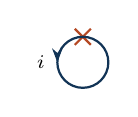
\begin{tikzpicture}[fcidiagram]
  \node[fvtx] (f) at (0,0.9) {};
  \draw[hloop] (0.45,0.45) arc (0:360:0.45);
  \node[dlab,left] at (-0.5,0.45) {$i$};
\end{tikzpicture}
&
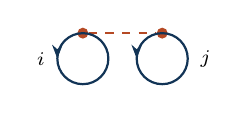
\begin{tikzpicture}[fcidiagram]
  \node[vtx] (v1) at (0,0) {}; \node[vtx] (v2) at (1.4,0) {}; \draw[vint] (v1) -- (v2);
  \draw[hloop] (0,-0.45) ++(0.45,0) arc (0:360:0.45);
  \draw[hloop] (1.4,-0.45) ++(0.45,0) arc (0:360:0.45);
  \node[dlab,left] at (-0.5,-0.45) {$i$}; \node[dlab,right] at (1.9,-0.45) {$j$};
\end{tikzpicture}
&
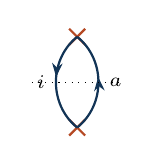
\begin{tikzpicture}[fcidiagram]
  \node[fvtx] (f1) at (0,0) {}; \node[fvtx] (f2) at (0,1.6) {};
  \draw[pline] (f1.center) .. controls (0.5,0.4) and (0.5,1.2) .. (f2.center);
  \draw[hline] (f1.center) .. controls (-0.5,0.4) and (-0.5,1.2) .. (f2.center);
  \draw[dotted] (-0.8,0.8) -- (0.8,0.8);
  \node[dlab,left] at (-0.4,0.8) {$i$}; \node[dlab,right] at (0.4,0.8) {$a$};
\end{tikzpicture}
&
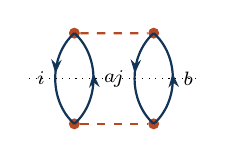
\begin{tikzpicture}[fcidiagram]
  \node[vtx] (b1) at (0,0) {}; \node[vtx] (b2) at (1.4,0) {}; \draw[vint] (b1) -- (b2);
  \node[vtx] (t1) at (0,1.6) {}; \node[vtx] (t2) at (1.4,1.6) {}; \draw[vint] (t1) -- (t2);
  \draw[pline] (b1.center) .. controls (0.45,0.4) and (0.45,1.2) .. (t1.center);
  \draw[hline] (b1.center) .. controls (-0.45,0.4) and (-0.45,1.2) .. (t1.center);
  \draw[pline] (b2.center) .. controls (1.85,0.4) and (1.85,1.2) .. (t2.center);
  \draw[hline] (b2.center) .. controls (0.95,0.4) and (0.95,1.2) .. (t2.center);
  \draw[dotted] (-0.8,0.8) -- (2.2,0.8);
  \node[dlab,left] at (-0.35,0.8) {$i$}; \node[dlab,right] at (0.35,0.8) {$a$};
  \node[dlab,left] at (1.05,0.8) {$j$}; \node[dlab,right] at (1.75,0.8) {$b$};
\end{tikzpicture}\\[0.3em]
$\sum_i u_{ii}$ & $\tfrac12\sum_{ij}\vbar{i}{j}{i}{j}$ & $\sum_{ia}\dfrac{\ftil{ia}\ftil{ai}}{\varepsilon_i-\varepsilon_a}$ & $\tfrac14\sum_{ijab}\dfrac{|\vbar{a}{b}{i}{j}|^2}{\varepsilon_i+\varepsilon_j-\varepsilon_a-\varepsilon_b}$
\end{tabular}
\end{center}
\begin{itemize}
\item First order (bare vertices, bubbles drawn): \(h=l=1\) and \(h=l=2\) with one equivalent pair, no cut: both \(+\). Together \(\Eref-\varepsilon_0\).
\item Second order (normal-ordered vertices): the two diagrams of pause \#3.
\item \alert{Hartree-Fock basis}: \(f\) is diagonal with eigenvalues \(\varepsilon_p\), so \(\ftil{pq}=0\) for all \(p,q\): every cross vanishes, every bubble with it (Brillouin), and only the ring survives -- MP2. Pairing model: \(\ftil{ai}=0\) for any basis, ring \(=-\tfrac{7}{24}g^2\).
\end{itemize}
\end{frame}

% ======================================================================
\section{Friday, lecture 3: Third order}
% ======================================================================

\begin{frame}[shrink=12]{Enumerating the third order by intermediate states}
\(E^{(3)}=\av{WR_0WR_0W}\): all connected drawings with three normal-ordered vertices. The intermediate states can only be \alert{singles} (S) or \alert{doubles} (D):
\begin{itemize}
\item Bottom vertex on the reference: a cross creates a single (\(\ftil{ai}\)), an interaction a double (\(\vbar{a}{b}{i}{j}\)) -- a normal-ordered operator has to \emph{create} every line it touches.
\item Top vertex: a cross closes a single (\(\ftil{ia}\)), an interaction a double (\(\vbar{i}{j}{a}{b}\)).
\item Middle vertex: S\(\to\)S, S\(\to\)D, D\(\to\)S, D\(\to\)D, by a cross or by an interaction. Triples and quadruples cannot be closed by the top vertex; a return to the reference is killed by \(Q\).
\end{itemize}
\begin{center}\scriptsize
\begin{tabular}{clllc}
\toprule
& vertices (bottom to top) & states & description & sign, weight\\
\midrule
1, 2 & cross, cross, cross & S, S & particle-line insertion / hole-line insertion & \(+\) / \(-\)\\
3 & cross, cross, interaction & S, D & two pairs created by crosses & \(+\)\\
4 & cross, interaction, cross & S, S & particle-hole scattering & \(-\)\\
5, 6 & cross, interaction, interaction & S, D & particle line / hole line into the interaction & \(+\tfrac12\) / \(-\tfrac12\)\\
7, 8 & interaction, cross, interaction & D, D & particle-line / hole-line insertion & \(+\tfrac12\) / \(-\tfrac12\)\\
9 & interaction, cross, cross & D, S & two pairs closed by crosses & \(+\)\\
10, 11 & interaction, interaction, interaction & D, D & particle-particle ladder / hole-hole ladder & \(+\tfrac18\) / \(+\tfrac18\)\\
12 & interaction, interaction, interaction & D, D & particle-hole ring & \(-\)\\
13, 14 & interaction, interaction, cross & D, S & particle lines / hole lines into the interaction & \(+\tfrac12\) / \(-\tfrac12\)\\
\bottomrule
\end{tabular}
\end{center}
\alert{Fourteen diagrams.} Nothing forgotten, nothing counted twice: that is what the pictures are for.
\end{frame}

\begin{frame}[shrink=10]{The three diagrams with three interactions: MP3}
\begin{center}
\begin{tabular}{@{}c@{\hspace{3.5em}}c@{\hspace{3.5em}}c@{}}
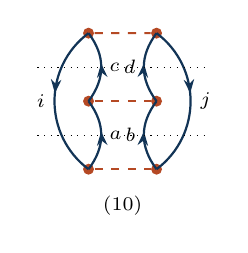
\begin{tikzpicture}[fcidiagram]
  \node[vtx] (b1) at (0,0) {}; \node[vtx] (b2) at (1.2,0) {}; \draw[vint] (b1) -- (b2);
  \node[vtx] (m1) at (0,1.2) {}; \node[vtx] (m2) at (1.2,1.2) {}; \draw[vint] (m1) -- (m2);
  \node[vtx] (t1) at (0,2.4) {}; \node[vtx] (t2) at (1.2,2.4) {}; \draw[vint] (t1) -- (t2);
  \draw[pline] (b1.center) .. controls (0.3,0.4) and (0.3,0.8) .. (m1.center);
  \draw[pline] (b2.center) .. controls (0.9,0.4) and (0.9,0.8) .. (m2.center);
  \draw[pline] (m1.center) .. controls (0.3,1.6) and (0.3,2.0) .. (t1.center);
  \draw[pline] (m2.center) .. controls (0.9,1.6) and (0.9,2.0) .. (t2.center);
  \draw[hline] (b1.center) .. controls (-0.8,0.6) and (-0.8,1.8) .. (t1.center);
  \draw[hline] (b2.center) .. controls (2.0,0.6) and (2.0,1.8) .. (t2.center);
  \draw[dotted] (-0.9,0.6) -- (2.1,0.6); \draw[dotted] (-0.9,1.8) -- (2.1,1.8);
  \node[dlab,right] at (0.2,0.6) {$a$}; \node[dlab,left] at (1.0,0.6) {$b$};
  \node[dlab,right] at (0.2,1.8) {$c$}; \node[dlab,left] at (1.0,1.8) {$d$};
  \node[dlab,left] at (-0.6,1.2) {$i$}; \node[dlab,right] at (1.8,1.2) {$j$};
  \node[dlab,below] at (0.6,-0.3) {(10)};
\end{tikzpicture}
&
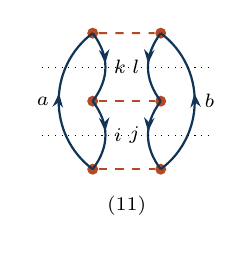
\begin{tikzpicture}[fcidiagram]
  \node[vtx] (b1) at (0,0) {}; \node[vtx] (b2) at (1.2,0) {}; \draw[vint] (b1) -- (b2);
  \node[vtx] (m1) at (0,1.2) {}; \node[vtx] (m2) at (1.2,1.2) {}; \draw[vint] (m1) -- (m2);
  \node[vtx] (t1) at (0,2.4) {}; \node[vtx] (t2) at (1.2,2.4) {}; \draw[vint] (t1) -- (t2);
  \draw[hline] (b1.center) .. controls (0.3,0.4) and (0.3,0.8) .. (m1.center);
  \draw[hline] (b2.center) .. controls (0.9,0.4) and (0.9,0.8) .. (m2.center);
  \draw[hline] (m1.center) .. controls (0.3,1.6) and (0.3,2.0) .. (t1.center);
  \draw[hline] (m2.center) .. controls (0.9,1.6) and (0.9,2.0) .. (t2.center);
  \draw[pline] (b1.center) .. controls (-0.8,0.6) and (-0.8,1.8) .. (t1.center);
  \draw[pline] (b2.center) .. controls (2.0,0.6) and (2.0,1.8) .. (t2.center);
  \draw[dotted] (-0.9,0.6) -- (2.1,0.6); \draw[dotted] (-0.9,1.8) -- (2.1,1.8);
  \node[dlab,right] at (0.2,0.6) {$i$}; \node[dlab,left] at (1.0,0.6) {$j$};
  \node[dlab,right] at (0.2,1.8) {$k$}; \node[dlab,left] at (1.0,1.8) {$l$};
  \node[dlab,left] at (-0.6,1.2) {$a$}; \node[dlab,right] at (1.8,1.2) {$b$};
  \node[dlab,below] at (0.6,-0.3) {(11)};
\end{tikzpicture}
&
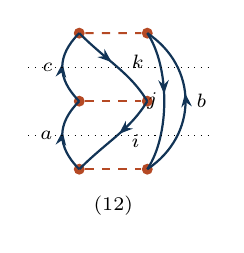
\begin{tikzpicture}[fcidiagram]
  \node[vtx] (b1) at (0,0) {}; \node[vtx] (b2) at (1.2,0) {}; \draw[vint] (b1) -- (b2);
  \node[vtx] (m1) at (0,1.2) {}; \node[vtx] (m2) at (1.2,1.2) {}; \draw[vint] (m1) -- (m2);
  \node[vtx] (t1) at (0,2.4) {}; \node[vtx] (t2) at (1.2,2.4) {}; \draw[vint] (t1) -- (t2);
  \draw[pline] (b1.center) .. controls (-0.4,0.4) and (-0.4,0.8) .. (m1.center);
  \draw[pline] (m1.center) .. controls (-0.4,1.6) and (-0.4,2.0) .. (t1.center);
  \draw[hline] (b1.center) .. controls (0.5,0.5) and (0.9,0.7) .. (m2.center);
  \draw[hline] (m2.center) .. controls (0.9,1.7) and (0.5,1.9) .. (t1.center);
  \draw[pline] (b2.center) .. controls (2.1,0.6) and (2.1,1.8) .. (t2.center);
  \draw[hline] (b2.center) .. controls (1.6,0.6) and (1.6,1.8) .. (t2.center);
  \draw[dotted] (-0.9,0.6) -- (2.3,0.6); \draw[dotted] (-0.9,1.8) -- (2.3,1.8);
  \node[dlab,left] at (-0.3,0.6) {$a$}; \node[dlab,left] at (-0.3,1.8) {$c$};
  \node[dlab,right] at (0.75,0.5) {$i$}; \node[dlab,right] at (0.75,1.9) {$k$};
  \node[dlab,right] at (1.9,1.2) {$b$}; \node[dlab,left] at (1.55,1.2) {$j$};
  \node[dlab,below] at (0.6,-0.3) {(12)};
\end{tikzpicture}
\end{tabular}
\end{center}
\[
\Delta E^{(3)}_{\rm MP}=
\frac18\sum\frac{\vbar{i}{j}{c}{d}\vbar{c}{d}{a}{b}\vbar{a}{b}{i}{j}}{\varepsilon_{ij}^{ab}\,\varepsilon_{ij}^{cd}}
+\frac18\sum\frac{\vbar{k}{l}{a}{b}\vbar{i}{j}{k}{l}\vbar{a}{b}{i}{j}}{\varepsilon_{ij}^{ab}\,\varepsilon_{kl}^{ab}}
+\sum\frac{\vbar{k}{j}{c}{b}\vbar{i}{c}{a}{k}\vbar{a}{b}{i}{j}}{\varepsilon_{ij}^{ab}\,\varepsilon_{kj}^{cb}},
\]
\centerline{\small with \(\varepsilon_{ij}^{ab}\equiv\varepsilon_i+\varepsilon_j-\varepsilon_a-\varepsilon_b\).}
\small Ladders: three pairs of equivalent lines, \(\tfrac18\); \(h=2\) or \(4\), \(l=2\): \(+\). Ring: no equivalent lines, \(h=3\), \(l=2\): \(-\) in front of \(\vbar{c}{i}{a}{k}\), i.e.\ \(+\) with \(\vbar{i}{c}{a}{k}\).
\end{frame}

\begin{frame}{MP3: what the three diagrams say}
\begin{itemize}
\item In a canonical Hartree-Fock basis \(\ftil{pq}=f_{pq}-\varepsilon_p\delta_{pq}=0\): every diagram with a cross vanishes, and the three are the \emph{only} third-order diagrams -- the M\o{}ller-Plesset third-order energy.
\item Particle-particle ladder: the two excited particles scatter off each other once before they fall back. Hole-hole ladder: the same for the two holes. Ring: one particle-hole pair scatters into another.
\item Each is the third-order member of an infinite family. Ladders of every length: Brueckner's \(G\)-matrix of nuclear physics. Rings of every length: the RPA of chapter 7 (week 40, and the stability matrix of week 39). Both at once, with the terms that mix them: coupled-cluster doubles, chapter 10.
\end{itemize}
\mbbox{Why one may sum a family to all orders and still get a meaningful answer is the content of the linked-diagram theorem (lecture 4): the pieces being summed are the ones that count, and no unlinked piece sneaks in.}
\end{frame}

\begin{frame}{The eleven diagrams with at least one cross}
\begin{center}
\scalebox{0.74}{\begin{tabular}{@{}c@{\hspace{2.2em}}c@{\hspace{2.2em}}c@{\hspace{2.2em}}c@{}}
% 1: F F F particle insertion
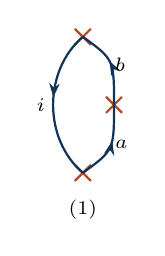
\begin{tikzpicture}[fcidiagram]
  \node[fvtx] (b) at (0,0) {}; \node[fvtx] (m) at (0.55,1.2) {}; \node[fvtx] (t) at (0,2.4) {};
  \draw[hline] (b.center) .. controls (-0.7,0.6) and (-0.7,1.8) .. (t.center);
  \draw[pline] (b.center) .. controls (0.55,0.4) .. (m.center);
  \draw[pline] (m.center) .. controls (0.55,2.0) .. (t.center);
  \node[dlab,left] at (-0.5,1.2) {$i$}; \node[dlab,right] at (0.4,0.5) {$a$}; \node[dlab,right] at (0.4,1.9) {$b$};
  \node[dlab,below] at (0,-0.3) {(1)};
\end{tikzpicture}
&
% 2: F F F hole insertion
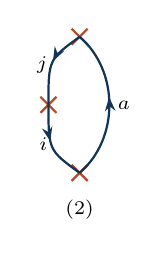
\begin{tikzpicture}[fcidiagram]
  \node[fvtx] (b) at (0,0) {}; \node[fvtx] (m) at (-0.55,1.2) {}; \node[fvtx] (t) at (0,2.4) {};
  \draw[pline] (b.center) .. controls (0.7,0.6) and (0.7,1.8) .. (t.center);
  \draw[hline] (b.center) .. controls (-0.55,0.4) .. (m.center);
  \draw[hline] (m.center) .. controls (-0.55,2.0) .. (t.center);
  \node[dlab,right] at (0.5,1.2) {$a$}; \node[dlab,left] at (-0.4,0.5) {$i$}; \node[dlab,left] at (-0.4,1.9) {$j$};
  \node[dlab,below] at (0,-0.3) {(2)};
\end{tikzpicture}
&
% 3: F F V
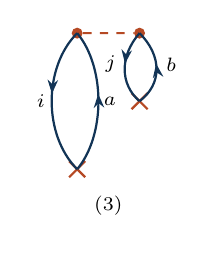
\begin{tikzpicture}[fcidiagram]
  \node[fvtx] (b) at (0,0) {}; \node[fvtx] (m) at (1.1,1.2) {};
  \node[vtx] (t1) at (0,2.4) {}; \node[vtx] (t2) at (1.1,2.4) {}; \draw[vint] (t1) -- (t2);
  \draw[hline] (b.center) .. controls (-0.6,0.6) and (-0.6,1.8) .. (t1.center);
  \draw[pline] (b.center) .. controls (0.5,0.6) and (0.5,1.8) .. (t1.center);
  \draw[hline] (m.center) .. controls (0.75,1.5) and (0.75,2.0) .. (t2.center);
  \draw[pline] (m.center) .. controls (1.5,1.5) and (1.5,2.0) .. (t2.center);
  \node[dlab,left] at (-0.4,1.2) {$i$}; \node[dlab,right] at (0.3,1.2) {$a$};
  \node[dlab,left] at (0.85,1.85) {$j$}; \node[dlab,right] at (1.4,1.85) {$b$};
  \node[dlab,below] at (0.55,-0.3) {(3)};
\end{tikzpicture}
&
% 4: F V F
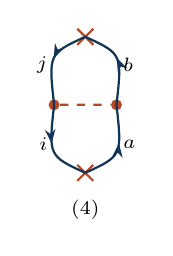
\begin{tikzpicture}[fcidiagram]
  \node[fvtx] (b) at (0.55,0) {}; \node[fvtx] (t) at (0.55,2.4) {};
  \node[vtx] (m1) at (0,1.2) {}; \node[vtx] (m2) at (1.1,1.2) {}; \draw[vint] (m1) -- (m2);
  \draw[hline] (b.center) .. controls (-0.1,0.3) .. (m1.center);
  \draw[pline] (b.center) .. controls (1.2,0.3) .. (m2.center);
  \draw[hline] (m1.center) .. controls (-0.1,2.1) .. (t.center);
  \draw[pline] (m2.center) .. controls (1.2,2.1) .. (t.center);
  \node[dlab,left] at (0.05,0.5) {$i$}; \node[dlab,right] at (1.05,0.5) {$a$};
  \node[dlab,left] at (0.05,1.9) {$j$}; \node[dlab,right] at (1.05,1.9) {$b$};
  \node[dlab,below] at (0.55,-0.3) {(4)};
\end{tikzpicture}
\\[1.2em]
% 5: F V V particle into V
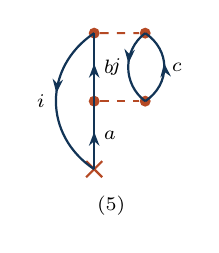
\begin{tikzpicture}[fcidiagram]
  \node[fvtx] (b) at (0.3,0) {};
  \node[vtx] (m1) at (0.3,1.2) {}; \node[vtx] (m2) at (1.2,1.2) {}; \draw[vint] (m1) -- (m2);
  \node[vtx] (t1) at (0.3,2.4) {}; \node[vtx] (t2) at (1.2,2.4) {}; \draw[vint] (t1) -- (t2);
  \draw[hline] (b.center) .. controls (-0.6,0.6) and (-0.6,1.8) .. (t1.center);
  \draw[pline] (b.center) -- (m1.center); \draw[pline] (m1.center) -- (t1.center);
  \draw[pline] (m2.center) .. controls (1.65,1.5) and (1.65,2.1) .. (t2.center);
  \draw[hline] (m2.center) .. controls (0.8,1.5) and (0.8,2.1) .. (t2.center);
  \node[dlab,left] at (-0.4,1.2) {$i$}; \node[dlab,right] at (0.3,0.6) {$a$}; \node[dlab,right] at (0.3,1.8) {$b$};
  \node[dlab,right] at (1.5,1.8) {$c$}; \node[dlab,left] at (0.95,1.8) {$j$};
  \node[dlab,below] at (0.6,-0.3) {(5)};
\end{tikzpicture}
&
% 6: F V V hole into V
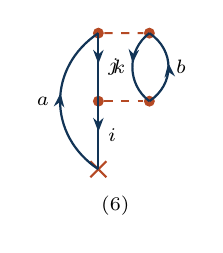
\begin{tikzpicture}[fcidiagram]
  \node[fvtx] (b) at (0.3,0) {};
  \node[vtx] (m1) at (0.3,1.2) {}; \node[vtx] (m2) at (1.2,1.2) {}; \draw[vint] (m1) -- (m2);
  \node[vtx] (t1) at (0.3,2.4) {}; \node[vtx] (t2) at (1.2,2.4) {}; \draw[vint] (t1) -- (t2);
  \draw[pline] (b.center) .. controls (-0.6,0.6) and (-0.6,1.8) .. (t1.center);
  \draw[hline] (b.center) -- (m1.center); \draw[hline] (m1.center) -- (t1.center);
  \draw[pline] (m2.center) .. controls (1.65,1.5) and (1.65,2.1) .. (t2.center);
  \draw[hline] (m2.center) .. controls (0.8,1.5) and (0.8,2.1) .. (t2.center);
  \node[dlab,left] at (-0.4,1.2) {$a$}; \node[dlab,right] at (0.3,0.6) {$i$}; \node[dlab,right] at (0.3,1.8) {$j$};
  \node[dlab,right] at (1.5,1.8) {$b$}; \node[dlab,left] at (0.95,1.8) {$k$};
  \node[dlab,below] at (0.6,-0.3) {(6)};
\end{tikzpicture}
&
% 7: V F V particle insertion
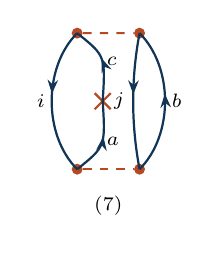
\begin{tikzpicture}[fcidiagram]
  \node[vtx] (b1) at (0,0) {}; \node[vtx] (b2) at (1.1,0) {}; \draw[vint] (b1) -- (b2);
  \node[vtx] (t1) at (0,2.4) {}; \node[vtx] (t2) at (1.1,2.4) {}; \draw[vint] (t1) -- (t2);
  \node[fvtx] (m) at (0.45,1.2) {};
  \draw[hline] (b1.center) .. controls (-0.6,0.6) and (-0.6,1.8) .. (t1.center);
  \draw[pline] (b1.center) .. controls (0.5,0.4) .. (m.center);
  \draw[pline] (m.center) .. controls (0.5,2.0) .. (t1.center);
  \draw[pline] (b2.center) .. controls (1.7,0.6) and (1.7,1.8) .. (t2.center);
  \draw[hline] (b2.center) .. controls (0.95,0.8) and (0.95,1.6) .. (t2.center);
  \node[dlab,left] at (-0.4,1.2) {$i$}; \node[dlab,right] at (0.35,0.5) {$a$}; \node[dlab,right] at (0.35,1.9) {$c$};
  \node[dlab,right] at (1.5,1.2) {$b$}; \node[dlab,left] at (1.0,1.2) {$j$};
  \node[dlab,below] at (0.55,-0.3) {(7)};
\end{tikzpicture}
&
% 8: V F V hole insertion
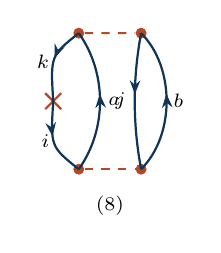
\begin{tikzpicture}[fcidiagram]
  \node[vtx] (b1) at (0,0) {}; \node[vtx] (b2) at (1.1,0) {}; \draw[vint] (b1) -- (b2);
  \node[vtx] (t1) at (0,2.4) {}; \node[vtx] (t2) at (1.1,2.4) {}; \draw[vint] (t1) -- (t2);
  \node[fvtx] (m) at (-0.45,1.2) {};
  \draw[pline] (b1.center) .. controls (0.5,0.7) and (0.5,1.7) .. (t1.center);
  \draw[hline] (b1.center) .. controls (-0.5,0.4) .. (m.center);
  \draw[hline] (m.center) .. controls (-0.5,2.0) .. (t1.center);
  \draw[pline] (b2.center) .. controls (1.7,0.6) and (1.7,1.8) .. (t2.center);
  \draw[hline] (b2.center) .. controls (0.95,0.8) and (0.95,1.6) .. (t2.center);
  \node[dlab,right] at (0.35,1.2) {$a$}; \node[dlab,left] at (-0.35,0.5) {$i$}; \node[dlab,left] at (-0.35,1.9) {$k$};
  \node[dlab,right] at (1.5,1.2) {$b$}; \node[dlab,left] at (1.0,1.2) {$j$};
  \node[dlab,below] at (0.55,-0.3) {(8)};
\end{tikzpicture}
\\[1.2em]
% 9: V F F
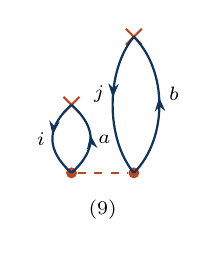
\begin{tikzpicture}[fcidiagram]
  \node[vtx] (b1) at (0,0) {}; \node[vtx] (b2) at (1.1,0) {}; \draw[vint] (b1) -- (b2);
  \node[fvtx] (m) at (0,1.2) {}; \node[fvtx] (t) at (1.1,2.4) {};
  \draw[hline] (b1.center) .. controls (-0.45,0.4) and (-0.45,0.8) .. (m.center);
  \draw[pline] (b1.center) .. controls (0.45,0.4) and (0.45,0.8) .. (m.center);
  \draw[hline] (b2.center) .. controls (0.6,0.6) and (0.6,1.8) .. (t.center);
  \draw[pline] (b2.center) .. controls (1.7,0.6) and (1.7,1.8) .. (t.center);
  \node[dlab,left] at (-0.3,0.6) {$i$}; \node[dlab,right] at (0.3,0.6) {$a$};
  \node[dlab,left] at (0.75,1.4) {$j$}; \node[dlab,right] at (1.55,1.4) {$b$};
  \node[dlab,below] at (0.55,-0.3) {(9)};
\end{tikzpicture}
&
% 13: V V F particles into V
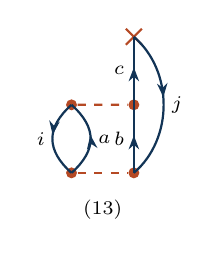
\begin{tikzpicture}[fcidiagram]
  \node[vtx] (b1) at (0,0) {}; \node[vtx] (b2) at (1.1,0) {}; \draw[vint] (b1) -- (b2);
  \node[vtx] (m1) at (0,1.2) {}; \node[vtx] (m2) at (1.1,1.2) {}; \draw[vint] (m1) -- (m2);
  \node[fvtx] (t) at (1.1,2.4) {};
  \draw[hline] (b1.center) .. controls (-0.45,0.4) and (-0.45,0.8) .. (m1.center);
  \draw[pline] (b1.center) .. controls (0.45,0.4) and (0.45,0.8) .. (m1.center);
  \draw[pline] (b2.center) -- (m2.center); \draw[pline] (m2.center) -- (t.center);
  \draw[hline] (b2.center) .. controls (1.8,0.6) and (1.8,1.8) .. (t.center);
  \node[dlab,left] at (-0.3,0.6) {$i$}; \node[dlab,right] at (0.3,0.6) {$a$};
  \node[dlab,left] at (1.1,0.6) {$b$}; \node[dlab,left] at (1.1,1.8) {$c$}; \node[dlab,right] at (1.6,1.2) {$j$};
  \node[dlab,below] at (0.55,-0.3) {(13)};
\end{tikzpicture}
&
% 14: V V F holes into V
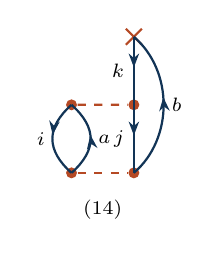
\begin{tikzpicture}[fcidiagram]
  \node[vtx] (b1) at (0,0) {}; \node[vtx] (b2) at (1.1,0) {}; \draw[vint] (b1) -- (b2);
  \node[vtx] (m1) at (0,1.2) {}; \node[vtx] (m2) at (1.1,1.2) {}; \draw[vint] (m1) -- (m2);
  \node[fvtx] (t) at (1.1,2.4) {};
  \draw[hline] (b1.center) .. controls (-0.45,0.4) and (-0.45,0.8) .. (m1.center);
  \draw[pline] (b1.center) .. controls (0.45,0.4) and (0.45,0.8) .. (m1.center);
  \draw[hline] (b2.center) -- (m2.center); \draw[hline] (m2.center) -- (t.center);
  \draw[pline] (b2.center) .. controls (1.8,0.6) and (1.8,1.8) .. (t.center);
  \node[dlab,left] at (-0.3,0.6) {$i$}; \node[dlab,right] at (0.3,0.6) {$a$};
  \node[dlab,left] at (1.1,0.6) {$j$}; \node[dlab,left] at (1.1,1.8) {$k$}; \node[dlab,right] at (1.6,1.2) {$b$};
  \node[dlab,below] at (0.55,-0.3) {(14)};
\end{tikzpicture}
&
\\
\end{tabular}}
\end{center}
\small All vanish in a canonical HF basis. In the models of chapter 9 (\(H_0\) diagonal by construction, reference not HF) the cross is the bubble \(U_{pq}\): 7 and 8 are the first self-energy insertions on a particle and a hole line. Mirror images in time: 3/9, 5/13, 6/14.
\end{frame}

\begin{frame}[shrink=8]{The full third order, read off the drawings: diagrams 1--7}
\begin{align*}
E^{(3)}
={}& \sum_{iab}\frac{\ftil{ib}\ftil{ba}\ftil{ai}}{(\varepsilon_i-\varepsilon_a)(\varepsilon_i-\varepsilon_b)}
 - \sum_{ija}\frac{\ftil{ja}\ftil{ij}\ftil{ai}}{(\varepsilon_i-\varepsilon_a)(\varepsilon_j-\varepsilon_a)}
 + \sum_{ijab}\frac{\vbar{i}{j}{a}{b}\ftil{bj}\ftil{ai}}{(\varepsilon_i-\varepsilon_a)\,\varepsilon_{ij}^{ab}}\\
&- \sum_{ijab}\frac{\ftil{jb}\vbar{i}{b}{j}{a}\ftil{ai}}{(\varepsilon_i-\varepsilon_a)(\varepsilon_j-\varepsilon_b)}
 + \frac12\sum\frac{\vbar{i}{j}{b}{c}\vbar{b}{c}{a}{j}\ftil{ai}}{(\varepsilon_i-\varepsilon_a)\,\varepsilon_{ij}^{bc}}
 - \frac12\sum\frac{\vbar{j}{k}{a}{b}\vbar{i}{b}{j}{k}\ftil{ai}}{(\varepsilon_i-\varepsilon_a)\,\varepsilon_{jk}^{ab}}\\
&+ \frac12\sum\frac{\vbar{i}{j}{c}{b}\ftil{ca}\vbar{a}{b}{i}{j}}{\varepsilon_{ij}^{ab}\,\varepsilon_{ij}^{cb}}
 \ +\ \cdots\qquad(\varepsilon_{ij}^{ab}=\varepsilon_i+\varepsilon_j-\varepsilon_a-\varepsilon_b)
\end{align*}
\begin{block}{A sign worth checking: diagram 2, the cross on a hole line}
Ends \((a,i),(i,j),(j,a)\): \(\pi\) is one 3-cycle, \(l=1\); \(h=2\): sign \(-\). The cross adds a line, not a loop; whether the added line is a hole or a particle decides the sign -- the \(f_{ab}C_i^b\) versus \(-f_{ji}C_j^a\) of the singles equation of week 38. Diagram 1 (cross on the particle line) has the same single cycle but \(h=1\): \(+\).
\end{block}
\end{frame}

\begin{frame}[shrink=8]{The full third order, read off the drawings: diagrams 8--14}
\begin{align*}
\cdots
&- \frac12\sum\frac{\vbar{k}{j}{a}{b}\ftil{ik}\vbar{a}{b}{i}{j}}{\varepsilon_{ij}^{ab}\,\varepsilon_{kj}^{ab}}
 + \sum_{ijab}\frac{\ftil{jb}\ftil{ia}\vbar{a}{b}{i}{j}}{\varepsilon_{ij}^{ab}\,(\varepsilon_j-\varepsilon_b)}
 + \frac18\sum\frac{\vbar{i}{j}{c}{d}\vbar{c}{d}{a}{b}\vbar{a}{b}{i}{j}}{\varepsilon_{ij}^{ab}\,\varepsilon_{ij}^{cd}}\\
&+ \frac18\sum\frac{\vbar{k}{l}{a}{b}\vbar{i}{j}{k}{l}\vbar{a}{b}{i}{j}}{\varepsilon_{ij}^{ab}\,\varepsilon_{kl}^{ab}}
 - \sum\frac{\vbar{k}{j}{c}{b}\vbar{c}{i}{a}{k}\vbar{a}{b}{i}{j}}{\varepsilon_{ij}^{ab}\,\varepsilon_{kj}^{cb}}\\
&+ \frac12\sum\frac{\ftil{jc}\vbar{i}{c}{a}{b}\vbar{a}{b}{i}{j}}{\varepsilon_{ij}^{ab}\,(\varepsilon_j-\varepsilon_c)}
 - \frac12\sum\frac{\ftil{kb}\vbar{i}{j}{a}{k}\vbar{a}{b}{i}{j}}{\varepsilon_{ij}^{ab}\,(\varepsilon_k-\varepsilon_b)}.
\end{align*}
\begin{block}{A sign worth checking: diagram 12, the ring}
Ends \(1L{=}(a,i)\), \(1R{=}(b,j)\), \(2L{=}(c,a)\), \(2R{=}(i,k)\), \(3L{=}(k,c)\), \(3R{=}(j,b)\). Lines: \(1L\to2L\) (\(a\)), \(2L\to3L\) (\(c\)), \(3L\to2R\) (\(k\)), \(2R\to1L\) (\(i\)) -- one cycle; \(1R\to3R\) (\(b\)), \(3R\to1R\) (\(j\)) -- a second. \(l=2\), \(h=3\): \(-\) in front of \(\vbar{c}{i}{a}{k}\), which is \(+\) in front of \(\vbar{i}{c}{a}{k}\), the form usually quoted.
\end{block}
\end{frame}

\begin{frame}{Pause to think \#4}
\thinkq{4}{The pairing model: the interaction only moves a pair \((p\!\uparrow,p\!\downarrow)\to(q\!\uparrow,q\!\downarrow)\), \(H_0\) is diagonal by construction, \(u=0\).
\begin{enumerate}
\item Which of the fourteen diagrams can be non-zero? (Think: can the interaction connect the reference to a single? Can it scatter a particle and a hole from different pairs? What is \(\ftil{pq}=U_{pq}=\sum_j\vbar{p}{j}{q}{j}\) for an occupied and for an empty spin-orbital?)
\item Week 44 found principal \(-0.02300347\), renormalisation \(-0.01258681\), \(E^{(3)}=-0.01041667\) at \(g=0.5\). Guess which diagrams account for which number.
\end{enumerate}}
\end{frame}

\begin{frame}[shrink=12]{Answer to pause \#4}
\thinka{%
\begin{enumerate}
\item \(\ftil{ai}=0\) (a pair cannot be half moved) kills 1--6, 9, 13, 14; the ring needs a particle-hole scattering between different pairs and vanishes; \(U_{pp}=\vbar{p}{\bar p}{p}{\bar p}=-g/2\) for an \emph{occupied} spin-orbital, \(0\) for an empty one. Left: the two ladders and the hole insertion 8.
\item Four levels, two pairs, unit spacing: doubles \(i\to a\) with \(D_{ia}=2(\varepsilon_i-\varepsilon_a)=-4,-6,-2,-4\), element \(-g/2\).
{\normalsize\begin{align*}
\text{pp}&=-\tfrac{g^3}{8}\sum_i\Bigl(\sum_a\tfrac1{D_{ia}}\Bigr)^2=-\tfrac{53}{576}g^3,\qquad
\text{hh}=-\tfrac{53}{576}g^3,\\
\text{insertion}&=2\cdot\tfrac g2\sum_{ia}\tfrac{(g/2)^2}{D_{ia}^2}=+\tfrac{29}{288}g^3,
\qquad \boxed{E^{(3)}=-\tfrac{1}{12}g^3.}
\end{align*}}
At \(g=0.5\): \(-0.0115017-0.0115017+0.0125868=-0.0104167\). The ladders \emph{are} the principal term; the insertion \emph{is} minus the renormalisation term.
\end{enumerate}}
\end{frame}

\begin{frame}[shrink=14]{Where the ``correction larger than the answer'' went}
\begin{columns}[T]
\column{0.52\textwidth}
\begin{block}{In the bookkeeping of week 44}
The diagonal element \(V_{mm}\) of the middle vertex contains the reference energy \(V_{00}\); the renormalisation term subtracts it. What is left, \(W_{mm}=V_{mm}-V_{00}\), is the diagonal part of the ladders plus the mean-field insertions on the four lines of the double.
\end{block}
\begin{block}{Pairing model}
For a pair excitation the two cancel: \(W_{mm}=0\). So the hole insertion, \(+g\sum_m|V_{0m}|^2/D_m^2\) with \(-\ftil{ii}=g/2\) on each hole line, equals \(-V_{00}\sum_m|V_{0m}|^2/D_m^2\) exactly, and the principal term is the ladders alone.
\end{block}
\column{0.46\textwidth}
\numbox{\texttt{diagrams.py}, pairing \(g=0.5\):\\
pp ladder \(-0.011501736\)\\
hh ladder \(-0.011501736\)\\
hole insertion \(+0.012586806\)\\
sum \(-0.010416667=E^{(3)}\)\\[0.3em]
Pairing + particle-hole, \(g=0.5\), \(f=0.025\): ladders \(-0.0153905\) each, insertion \(+0.0169196\), ring \(0\), diagrams 2, 3, 5, 6, 9, 13, 14 switched on at \(\le1.5\times10^{-4}\) (\(O(f^2)\): two vertices only the particle-hole term supplies); sum \(-0.0138615=E^{(3)}\).}
\end{columns}
\small The renormalisation term was never a correlation correction: it removes a mean-field contribution. (The two ladders are equal because the model has as many empty levels as filled ones at the same spacing.)
\end{frame}

\begin{frame}[shrink=5]{The rules put to the test: a random Hamiltonian in which all fourteen are non-zero}
Eight spin-orbitals, four particles, \(\varepsilon_p\) increasing, random symmetric off-diagonal \(u_{pq}\), random Hermitian antisymmetrised \(\vbar{p}{q}{r}{s}\) (70 determinants). The fourteen diagrams are evaluated from the orbital-level elements with the rules; \(E^{(3)}\) from the recursion in the full determinant space.
\begin{center}\small
\begin{tabular}{lr@{\hspace{2em}}lr}
\toprule
1 particle insertion & \(0.029978687\) & 8 hole insertion & \(0.015920047\)\\
2 hole insertion & \(0.222374016\) & 9 \(V\) closed by two crosses & \(0.064812430\)\\
3 two crosses closed by \(V\) & \(0.064812430\) & 10 pp ladder & \(0.004426951\)\\
4 particle-hole scattering & \(0.152115743\) & 11 hh ladder & \(0.002250487\)\\
5 particle line into \(V\) & \(-0.023773776\) & 12 ph ring & \(0.008950096\)\\
6 hole line into \(V\) & \(-0.061323558\) & 13 \(V\) to single via particles & \(-0.023773776\)\\
7 particle insertion & \(0.004225746\) & 14 \(V\) to single via holes & \(-0.061323558\)\\
\midrule
sum of the fourteen & \(0.399671963\) & \(E^{(3)}\), determinant space & \(0.399671963\)\\
\bottomrule
\end{tabular}
\end{center}
\numbox{Agreement to \(10^{-12}\); principal \(-0.14176\), renormalisation \(-0.54143\), \(\av{WR_0WR_0W}=0.39967\). Second order: \((F,F)=-0.650749\), ring \(-0.146957\), sum \(=E^{(2)}=-0.797706\). A wrong sign or a wrong factor in any one of the fourteen would show up in the last line -- which is how diagram 4 was caught during the preparation of these slides.}
\end{frame}

\begin{frame}[fragile,shrink=10]{Reading a diagram into code: \texttt{diagrams.py}}
With \texttt{eps}, \texttt{ftil}, \texttt{vbar} and the occupied/empty index lists \texttt{o}, \texttt{v}; \texttt{D1[i,a]} \(=\varepsilon_i-\varepsilon_a\), \texttt{D2[i,j,a,b]} \(=\varepsilon_{ij}^{ab}\):
\begin{lstlisting}
v_oovv = vb[np.ix_(o, o, v, v)]   # <ij|v|ab>      v_vvoo = vb[np.ix_(v, v, o, o)]   # <ab|v|ij>
v_vvvv = vb[np.ix_(v, v, v, v)]   # <cd|v|ab>      v_oooo = vb[np.ix_(o, o, o, o)]   # <ij|v|kl>
v_vovo = vb[np.ix_(v, o, v, o)]   # <ci|v|ak>      foo, fov, fvo, fvv = blocks of ftil
# 10  particle-particle ladder: three equivalent pairs -> 1/8, h = 2, l = 2 -> +
pp   = 0.125 * np.einsum("ijcd,cdab,abij,ijab,ijcd->", v_oovv, v_vvvv, v_vvoo, 1/D2, 1/D2)
# 11  hole-hole ladder
hh   = 0.125 * np.einsum("klab,ijkl,abij,ijab,klab->", v_oovv, v_oooo, v_vvoo, 1/D2, 1/D2)
# 12  particle-hole ring: no equivalent lines, h = 3, l = 2 -> -
ring = -np.einsum("kjcb,ciak,abij,ijab,kjcb->", v_oovv, v_vovo, v_vvoo, 1/D2, 1/D2)
# 8   hole-line insertion on a double: one equivalent pair (a,b) -> 1/2, h = 3, l = 2 -> -
ins  = -0.5 * np.einsum("kjab,ik,abij,ijab,kjab->", v_oovv, foo, v_vvoo, 1/D2, 1/D2)
# 2   cross on a hole line: h = 2, l = 1 -> -
d2   = -np.einsum("ja,ij,ai,ia,ja->", fov, foo, fvo, 1/D1, 1/D1)
\end{lstlisting}
\small Each line is one diagram: the matrix elements in the order top to bottom, one \(1/D\) per cut, the weight and the sign in front. \texttt{GeneralHamiltonian} builds the same Hamiltonian in the determinant space and runs the recursion of week 44, so the two routes can be compared for any \((\varepsilon,u,\bar v)\). The notebook \texttt{week45.ipynb} is self-contained and repeats every number on these frames.
\end{frame}

% ======================================================================
\section{Friday, lecture 4: Unlinked diagrams and the linked-diagram theorem}
% ======================================================================

\begin{frame}{Fourth order: a new kind of drawing}
\[
E^{(4)}=\av{WR_0WR_0WR_0W}-E^{(2)}\av{WR_0^2W}.
\]
With four normal-ordered vertices a complete contraction can fall into \alert{two closed pieces of two vertices each}:
\begin{center}
\begin{tabular}{lll}
\toprule
pairing of vertices & intermediate states & \\
\midrule
\(1\)--\(3\) and \(2\)--\(4\) & \(m,\ m\otimes n,\ n\) & unlinked, overlapping in time\\
\(1\)--\(4\) and \(2\)--\(3\) & \(m,\ m\otimes n,\ m\) & unlinked, overlapping in time\\
\(1\)--\(2\) and \(3\)--\(4\) & \(m,\ \ph,\ n\) & \alert{zero}: no line crosses the middle cut, \(Q\) kills it\\
\bottomrule
\end{tabular}
\end{center}
\begin{itemize}
\item Each piece is a closed second-order diagram -- a ring, or two crosses.
\item Such a drawing is \alert{unlinked}: it contains a closed part with no line connecting it to the rest.
\item Everything else with four vertices is connected; the question is what the unlinked ones are worth.
\end{itemize}
\end{frame}

\begin{frame}{The two unlinked time orderings, drawn}
\begin{center}
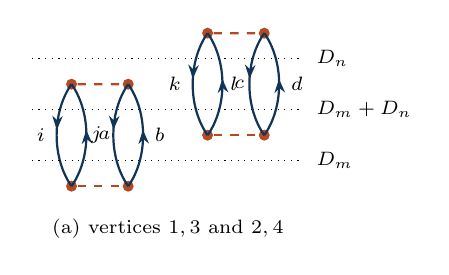
\begin{tikzpicture}[fcidiagram]
  % piece A: vertices 1 (y=0) and 3 (y=1.8); piece B: vertices 2 (y=0.9) and 4 (y=2.7)
  \node[vtx] (a1) at (0,0) {}; \node[vtx] (a2) at (1.0,0) {}; \draw[vint] (a1) -- (a2);
  \node[vtx] (a3) at (0,1.8) {}; \node[vtx] (a4) at (1.0,1.8) {}; \draw[vint] (a3) -- (a4);
  \draw[pline] (a1.center) .. controls (0.35,0.5) and (0.35,1.3) .. (a3.center);
  \draw[hline] (a1.center) .. controls (-0.35,0.5) and (-0.35,1.3) .. (a3.center);
  \draw[pline] (a2.center) .. controls (1.35,0.5) and (1.35,1.3) .. (a4.center);
  \draw[hline] (a2.center) .. controls (0.65,0.5) and (0.65,1.3) .. (a4.center);
  \node[vtx] (b1) at (2.4,0.9) {}; \node[vtx] (b2) at (3.4,0.9) {}; \draw[vint] (b1) -- (b2);
  \node[vtx] (b3) at (2.4,2.7) {}; \node[vtx] (b4) at (3.4,2.7) {}; \draw[vint] (b3) -- (b4);
  \draw[pline] (b1.center) .. controls (2.75,1.4) and (2.75,2.2) .. (b3.center);
  \draw[hline] (b1.center) .. controls (2.05,1.4) and (2.05,2.2) .. (b3.center);
  \draw[pline] (b2.center) .. controls (3.75,1.4) and (3.75,2.2) .. (b4.center);
  \draw[hline] (b2.center) .. controls (3.05,1.4) and (3.05,2.2) .. (b4.center);
  \draw[dotted] (-0.7,0.45) -- (4.1,0.45); \draw[dotted] (-0.7,1.35) -- (4.1,1.35); \draw[dotted] (-0.7,2.25) -- (4.1,2.25);
  \node[dlab,right] at (4.15,0.45) {$D_m$}; \node[dlab,right] at (4.15,1.35) {$D_m+D_n$}; \node[dlab,right] at (4.15,2.25) {$D_n$};
  \node[dlab,left] at (-0.3,0.9) {$i$}; \node[dlab,right] at (0.3,0.9) {$a$};
  \node[dlab,left] at (0.7,0.9) {$j$}; \node[dlab,right] at (1.3,0.9) {$b$};
  \node[dlab,left] at (2.1,1.8) {$k$}; \node[dlab,right] at (2.7,1.8) {$c$};
  \node[dlab,left] at (3.1,1.8) {$l$}; \node[dlab,right] at (3.7,1.8) {$d$};
  \node[dlab,below] at (1.7,-0.4) {(a) vertices $1,3$ and $2,4$};
\end{tikzpicture}
\hspace{2.5em}
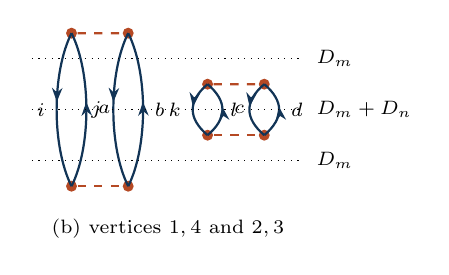
\begin{tikzpicture}[fcidiagram]
  % piece A: vertices 1 (y=0) and 4 (y=2.7); piece B: vertices 2 (y=0.9) and 3 (y=1.8)
  \node[vtx] (a1) at (0,0) {}; \node[vtx] (a2) at (1.0,0) {}; \draw[vint] (a1) -- (a2);
  \node[vtx] (a3) at (0,2.7) {}; \node[vtx] (a4) at (1.0,2.7) {}; \draw[vint] (a3) -- (a4);
  \draw[pline] (a1.center) .. controls (0.35,0.7) and (0.35,2.0) .. (a3.center);
  \draw[hline] (a1.center) .. controls (-0.35,0.7) and (-0.35,2.0) .. (a3.center);
  \draw[pline] (a2.center) .. controls (1.35,0.7) and (1.35,2.0) .. (a4.center);
  \draw[hline] (a2.center) .. controls (0.65,0.7) and (0.65,2.0) .. (a4.center);
  \node[vtx] (b1) at (2.4,0.9) {}; \node[vtx] (b2) at (3.4,0.9) {}; \draw[vint] (b1) -- (b2);
  \node[vtx] (b3) at (2.4,1.8) {}; \node[vtx] (b4) at (3.4,1.8) {}; \draw[vint] (b3) -- (b4);
  \draw[pline] (b1.center) .. controls (2.75,1.2) and (2.75,1.5) .. (b3.center);
  \draw[hline] (b1.center) .. controls (2.05,1.2) and (2.05,1.5) .. (b3.center);
  \draw[pline] (b2.center) .. controls (3.75,1.2) and (3.75,1.5) .. (b4.center);
  \draw[hline] (b2.center) .. controls (3.05,1.2) and (3.05,1.5) .. (b4.center);
  \draw[dotted] (-0.7,0.45) -- (4.1,0.45); \draw[dotted] (-0.7,1.35) -- (4.1,1.35); \draw[dotted] (-0.7,2.25) -- (4.1,2.25);
  \node[dlab,right] at (4.15,0.45) {$D_m$}; \node[dlab,right] at (4.15,1.35) {$D_m+D_n$}; \node[dlab,right] at (4.15,2.25) {$D_m$};
  \node[dlab,left] at (-0.3,1.35) {$i$}; \node[dlab,right] at (0.3,1.35) {$a$};
  \node[dlab,left] at (0.7,1.35) {$j$}; \node[dlab,right] at (1.3,1.35) {$b$};
  \node[dlab,left] at (2.1,1.35) {$k$}; \node[dlab,right] at (2.7,1.35) {$c$};
  \node[dlab,left] at (3.1,1.35) {$l$}; \node[dlab,right] at (3.7,1.35) {$d$};
  \node[dlab,below] at (1.7,-0.4) {(b) vertices $1,4$ and $2,3$};
\end{tikzpicture}
\end{center}
\small Two second-order rings, pairs \((ab,ij)\) and \((cd,kl)\) sharing no orbital; \(D_m=\varepsilon_{ij}^{ab}\), \(D_n=\varepsilon_{kl}^{cd}\) are the denominators of the rings on their own. The matrix elements, the weights and the signs of the two pieces simply \emph{multiply} (\((-1)^{h+l}\) is additive in \(h\) and \(l\)). Only the denominators are not local to a piece: in the middle both rings are open, and the energies \emph{add} because the excitations involve different orbitals.
\end{frame}

\begin{frame}[shrink=6]{The factorisation of the denominators}
Ordering (a): cuts \(D_m\), \(D_m+D_n\), \(D_n\). Ordering (b): \(D_m\), \(D_m+D_n\), \(D_m\). Add them:
\[
\boxed{\frac{1}{D_m(D_m+D_n)D_n}+\frac{1}{D_m(D_m+D_n)D_m}
=\frac{1}{D_m(D_m+D_n)}\cdot\frac{D_m+D_n}{D_mD_n}
=\frac{1}{D_m^2\,D_n}.}
\]
The sum over the two time orderings has \alert{factorised} into the product of the denominators of the two pieces, with the piece begun first counted twice. The two orderings with the roles exchanged give \(1/D_mD_n^2\).
\begin{block}{Compare with the folded term}
\[
E^{(2)}\av{WR_0^2W}=\sum_{m,n\ne0}\frac{W_{0n}W_{n0}}{D_n}\,\frac{W_{0m}W_{m0}}{D_m^2}
\]
-- exactly the sum of the unlinked diagrams, with the opposite sign.
\end{block}
\alert{The renormalisation term is not a correction to the principal term. It is the unlinked part of the principal term, counted once more with a minus sign, so that the two cancel and only the linked diagrams survive.}
\end{frame}

\begin{frame}[shrink=8]{The two-level benchmark of week 44, re-read}
Purely off-diagonal coupling \(\lambda\) between \(\ket{\Phi_1}\) and \(\ket{\Phi_2}\), \(V_{11}=V_{22}=0\):
\[
E^{(4)}=\underbrace{\av{VRVRVRV}}_{=0\ \text{since}\ QVQ=0}-E^{(2)}\av{VR^2V}=-\frac{\lambda^4}{D^3}>0 .
\]
\begin{columns}[T]
\column{0.5\textwidth}
\begin{block}{In diagram language}
With a single excited state there is \emph{no linked} fourth-order diagram. But there is an unlinked one: excite, de-excite, excite, de-excite -- the product of two second-order excursions, which \(Q\) does not kill because \dots
\end{block}
\column{0.48\textwidth}
\begin{alertblock}{\dots because?}
Because in a \emph{many-body} system the two excursions could overlap in time. Here they cannot (one state), so the unlinked piece in the principal term is absent, while the folded term still subtracts it. What the benchmark called ``the folded term is all there is'' is the theorem seen from its edge: the surviving term is a linked one -- an excitation of $\ket{\Phi_2}$ that is EPV in the many-body sense.
\end{alertblock}
\end{columns}
\vspace{0.4em}
\small This is also the origin of the quadratic scaling of pause \#1: a product of two closed pieces, each a sum over the whole system, grows like the square of the system size, and an energy cannot.
\end{frame}

\begin{frame}[shrink=5]{Two points of rigour}
\begin{columns}[T]
\column{0.5\textwidth}
\begin{block}{1. Exclusion-principle-violating terms}
If the two pieces share an orbital, the product state \(\ket{\Phi_m}\otimes\ket{\Phi_n}\) does not exist (Pauli), so the principal term lacks those terms while \(E^{(2)}\av{WR_0^2W}\) contains them. Goldstone's resolution: include the \emph{EPV} unlinked diagrams in the sum anyway -- they cancel the folded term -- and keep the linked diagrams that violate the exclusion principle in their intermediate states. The bookkeeping is consistent; the proof is next week.
\end{block}
\column{0.48\textwidth}
\begin{block}{2. The factorisation theorem (Frantz and Mills 1960)}
Shown here for two pieces of two vertices. In general: the sum over all relative time orderings of two pieces, each with its own cuts, equals the product of the two denominator products. Proved by induction on the number of vertices; it is the engine of the general proof.
\end{block}
\end{columns}
\vspace{0.3em}
\end{frame}

\begin{frame}{A numerical check: two non-interacting copies}
\numbox{Two non-interacting copies \(A\), \(B\) of a three-level pairing system with one pair each, \(g=0.5\) (no shared orbitals, no EPV terms). Restricting the intermediate states of the principal fourth-order term to \((A,AB,B)\), \((A,AB,A)\), \((B,AB,A)\), \((B,AB,B)\): \(-0.00183105\). \(2E^{(2)}_A\langle WR_0^2W\rangle_A\): \(-0.00183105\). \(E^{(4)}_{AB}=0.00109863=2E^{(4)}_A\) to fourteen digits. (\texttt{diagrams.py}, \texttt{fourth\_order\_unlinked}; the \((A,AB,B)\) and \((A,AB,A)\) orderings alone are \(-0.000437\) and \(-0.000478\) -- neither is a product, only their sum is.)}
\begin{itemize}
\item With disjoint orbitals the unperturbed energies add, \(D_{m\otimes n}=D_m+D_n\), and matrix elements and signs factorise; the \((A,AB,B)\) and \((A,AB,A)\) patterns have the denominators of the factorisation identity.
\item Their sum is \(\langle WR_0^2W\rangle_A\,E^{(2)}_B\); the other two give \(E^{(2)}_A\langle WR_0^2W\rangle_B\). The folded term of the two copies, \((E^{(2)}_A+E^{(2)}_B)(\langle WR_0^2W\rangle_A+\langle WR_0^2W\rangle_B)\), has exactly these cross terms: the cross-copy part of \(E^{(4)}\) cancels and \(E^{(4)}_{AB}=E^{(4)}_A+E^{(4)}_B\).
\end{itemize}
\end{frame}

\begin{frame}{Pause to think \#5}
\thinkq{3}{Brillouin-Wigner theory uses \(R_E=Q/(E_0-H_0)\): the \emph{exact} energy in every denominator, and no renormalisation terms at all.
\begin{enumerate}
\item Redo the factorisation identity with \(D_m\to D_m+\Delta E\), \(D_n\to D_n+\Delta E\), \(D_m+D_n\to D_m+D_n+\Delta E\). Does it still factorise?
\item What does this say about the unlinked diagrams of a truncated BW calculation, and about its scaling with system size?
\end{enumerate}}
\end{frame}

\begin{frame}{Answer to pause \#5}
\thinka{%
\begin{enumerate}
\item No. With \(d_m=D_m+\Delta E\) etc.\ the middle denominator is \(D_m+D_n+\Delta E\ne d_m+d_n\) (it is \(d_m+d_n-\Delta E\)), so \(\frac{1}{d_m(d_m+d_n-\Delta E)}\bigl(\frac1{d_n}+\frac1{d_m}\bigr)\ne\frac1{d_m^2d_n}\). The identity needs the \emph{unperturbed} energies, which add for disjoint excitations; the exact energy of the whole system does not split into pieces.
\item Nothing cancels: a BW calculation truncated at any finite number of vertices keeps its unlinked diagrams, which scale as (size)\(^2\) -- the table of week 44/chapter 9 (two copies: BW error \(\ne0\), RS error \(10^{-15}\)). Only the full resummation is exact, and it is as expensive as diagonalisation. This is the linked-diagram theorem's verdict on Brillouin-Wigner.
\end{enumerate}}
\end{frame}

\begin{frame}[shrink=5]{The linked-diagram theorem}
\begin{block}{Statement (Brueckner 1955, Goldstone 1957, Hugenholtz 1957)}
\[
\boxed{\Delta E=E^{(1)}+\sum_{n\ge1}\Bigl\langle W\bigl(R_0W\bigr)^{n-1}\Bigr\rangle_{\rm connected},
\qquad
\ket{\Psizero}=\sum_{n\ge0}\bigl(R_0W\bigr)^n\ket{\ph}\Big|_{\rm linked}.}
\]
The energy is the sum of all \alert{connected} closed diagrams, each evaluated with the four rules and \(R_0\) between successive vertices. The wave operator is the sum of all \alert{linked} diagrams: those with no closed disconnected part.
\end{block}
\begin{columns}[T]
\column{0.5\textwidth}
\begin{exampleblock}{Linked is not connected}
An open diagram may consist of two disconnected pieces \emph{each with open lines} -- two independent pair excitations, the product of two first-order doubles, the leading quadruple of \(\Psi^{(2)}\). Disconnected but linked: \alert{kept}.
\end{exampleblock}
\column{0.48\textwidth}
\begin{alertblock}{Unlinked}
A closed piece hanging loose -- a vacuum fluctuation -- multiplies the rest by a number that has nothing to do with the state. \alert{Removed}, by the renormalisation terms. For the energy, where all lines are closed, linked = connected (Goldstone's form).
\end{alertblock}
\end{columns}
\vspace{0.3em}
\small Seen so far: third order, nothing to subtract once the vertices are normal ordered; fourth order, the folded term removes the unlinked part. The general proof -- induction on the order, factorisation theorem as the engine, EPV terms included -- is week 46.
\end{frame}

\begin{frame}[shrink=10]{Three consequences}
\begin{enumerate}
\item \textbf{Size extensivity.} Every connected diagram is a single sum over the system and scales linearly with its size. This is the theorem behind the two-copies table (RS error \(10^{-15}\) at every order), and behind pause \#1.
\item \textbf{Brillouin-Wigner fails.} Its denominators contain \(E_0\) and do not factorise (pause \#5): a truncated BW energy keeps its unlinked diagrams and is not size extensive. Only RS -- equivalently, the linked-diagram expansion -- is used for many-body systems.
\item \textbf{Organise by topology, not by order.} The ladders and rings of third order are the first members of infinite families, each summable to all orders \emph{because} the theorem guarantees that the pieces one sums are the ones that count: Brueckner \(G\)-matrix (ladders), RPA (rings), and coupled cluster, whose \(\exp(T)\) generates exactly the disconnected-but-linked products of amplitudes that the wave-operator form of the theorem keeps. Chapter 10 proves the same statement -- the linked-cluster theorem -- by a different route.
\end{enumerate}
\mbbox{What the diagrams do \emph{not} do: make the series converge. The ladders and rings of the pairing model at \(g=2\) are drawn exactly as at \(g=0.5\), and the divergence table of week 44 is unchanged. The theorem is about \emph{which} terms, not about their size.}
\end{frame}

% ======================================================================
\section{Summary}
% ======================================================================

\begin{frame}[shrink=5]{Summary of week 45}
  \small
  \begin{columns}[T]
    \column{0.48\textwidth}
    \begin{block}{Thursday: the rules, derived}
      \begin{itemize}
        \item The complete lists: \(\Omega^{(1,2,3)}\), \(E^{(1,2,3,4)}\), renormalisation terms as products of pieces
        \item \(H_I=E^{(1)}+W\): the recursion in \(W\) has no \(E^{(1)}\) terms; \(E^{(3)}=\av{WR_0WR_0W}\), \(E^{(4)}=\av{WR_0WR_0WR_0W}-E^{(2)}\av{WR_0^2W}\)
        \item Contractions are lines (two non-zero contractions, arrows); cuts are denominators (\([H_0,\cre{p}]=\varepsilon_p\cre{p}\)); \(Q\) kills time-separated pieces only
        \item Weight: \(4^{n_V}\) relabellings against \((\tfrac14)^{n_V}\), equivalent lines halve the count. Sign: ends, \(\pi\), cycles = loops, \((-1)^{K-l}(-1)^p=(-1)^{h+l}\)
      \end{itemize}
    \end{block}
    \column{0.48\textwidth}
    \begin{block}{Friday: third order and the theorem}
      \begin{itemize}
        \item Fourteen connected third-order diagrams; MP3 = pp ladder + hh ladder + ph ring; pairing model \(-\tfrac{53}{576}-\tfrac{53}{576}+\tfrac{29}{288}=-\tfrac1{12}\) (\(g^3\)); all fourteen checked to \(10^{-12}\)
        \item Unlinked fourth-order diagrams; \(\frac{1}{D_m(D_m+D_n)D_n}+\frac{1}{D_m(D_m+D_n)D_m}=\frac{1}{D_m^2D_n}\); the folded term is the unlinked part with a minus sign
        \item Theorem: \(\Delta E\) = connected closed diagrams, \(\Psi_0\) = linked diagrams. Extensivity; BW does not factorise; sum by topology (ladders, rings, CC)
      \end{itemize}
    \end{block}
  \end{columns}
  \vspace{0.3em}
  \centering The renormalisation terms were never corrections: at third order they are the scalar part of a vertex, at fourth the unlinked diagrams -- in both cases something that was never there to begin with.
\end{frame}

\begin{frame}{Next week}
  \begin{exampleblock}{Week 46, November 12--13: the proof of the linked-diagram theorem}
    \small
    The factorisation theorem of Frantz and Mills in general -- the sum over all relative time orderings of two pieces equals the product of their denominator products -- proved by induction on the number of vertices; the exclusion-principle-violating diagrams and why they must be summed; the proof of the theorem by induction on the order, for the energy and for the wave operator; the wave-operator form and the disconnected-but-linked diagrams of $\Omega$; the time-dependent (Gell-Mann--Low) route as a second proof. Then the organisation by topology that follows: ladders, rings, and the step to coupled-cluster theory (chapter 10).
  \end{exampleblock}
  \vspace{0.5em}
  \small
  Reading: chapter 9, section 9.15; Shavitt and Bartlett, chapters 4--5 (and 6 for the time-dependent proof). The week-45 exercises (last frames, \texttt{Exercises/ExercisesWeek45.tex}) are discussed in the exercise session and answered on the week-46 slides.
\end{frame}

% ======================================================================
\section{Answers to the week-44 exercises}
% ======================================================================

\begin{frame}[shrink=8]{Exercise 1: the energy as a projection, and a)}
\(H=H_0+V\), \(H_0\ket{\phi_n}=\varepsilon_n\ket{\phi_n}\), \(H\ket{\psi_n}=E_n\ket{\psi_n}\); ground states non-degenerate and \(\braket{\phi_0}{\psi_0}\ne0\). Nothing is assumed about the norm of \(\ket{\psi_0}\).
\begin{block}{The projection}
Project \(H\ket{\psi_0}=E_0\ket{\psi_0}\) onto \(\bra{\phi_0}\); \(\bra{\phi_0}H_0=\varepsilon_0\bra{\phi_0}\) (Hermiticity), so
\[
(E_0-\varepsilon_0)\braket{\phi_0}{\psi_0}=\mel{\phi_0}{V}{\psi_0}
\quad\Longrightarrow\quad
\boxed{E_0-\varepsilon_0=\frac{\mel{\phi_0}{V}{\psi_0}}{\braket{\phi_0}{\psi_0}}.}
\]
Exact; a transition element, not an expectation value, hence not variational. Non-degeneracy is not needed here -- it is needed when \(z-H_0\) is inverted on the \(Q\) space.
\end{block}
\begin{block}{a) Idempotency}
\(P^2=\ket{\phi_0}\braket{\phi_0}{\phi_0}\bra{\phi_0}=P\); \(Q^2=(1-P)^2=1-2P+P^2=1-P=Q\). Also Hermitian, \(PQ=QP=0\), \(P+Q=1\), and \([P,H_0]=[Q,H_0]=0\) because \(\ket{\phi_0}\) is an eigenstate of \(H_0\): \(Q=\sum_{n\ne0}\ket{\phi_n}\bra{\phi_n}\), and any \(f(H_0)\) is diagonal in the same basis, so \(Qf(H_0)Q=Qf(H_0)=f(H_0)Q\) -- the licence to write \(Q/(z-H_0)\) (week 44, lecture 1).
\end{block}
\end{frame}

\begin{frame}[shrink=14]{Exercise 1 b): the expansion for arbitrary \(z\)}
\(\ket{\psi_0}=(P+Q)\ket{\psi_0}=\braket{\phi_0}{\psi_0}\ket{\phi_0}+Q\ket{\psi_0}\). Add and subtract \(z\ket{\psi_0}\) in the Schr\"odinger equation:
\[
(z-H_0)\ket{\psi_0}=(z-E_0+V)\ket{\psi_0}.
\]
Multiply by \(Q\); on the \(Q\) space \(z-H_0\) has eigenvalues \(z-\varepsilon_n\ne0\) (\(n\ne0\)) and can be inverted:
\[
\frac{Q}{z-H_0}\equiv Q(z-H_0)^{-1}Q=\sum_{n\ne0}\frac{\ket{\phi_n}\bra{\phi_n}}{z-\varepsilon_n},
\qquad
Q\ket{\psi_0}=\frac{Q}{z-H_0}(z-E_0+V)\ket{\psi_0}.
\]
(At \(z=\varepsilon_0\) the full inverse has a pole; the reduced one exists iff the ground state of \(H_0\) is non-degenerate -- \emph{this} is where the assumption enters.) Call \(A(z)=\frac{Q}{z-H_0}(z-E_0+V)\) and iterate:
\[
\ket{\psi_0}=\braket{\phi_0}{\psi_0}\bigl(1+A+\cdots+A^N\bigr)\ket{\phi_0}+A^{N+1}\ket{\psi_0}
\ \xrightarrow{N\to\infty}\
\boxed{\ket{\psi_0}=\braket{\phi_0}{\psi_0}\sum_{n=0}^\infty\Bigl(\frac{Q}{z-H_0}(z-E_0+V)\Bigr)^n\ket{\phi_0},}
\]
a formal Neumann series (convergence not guaranteed); the overlap is an overall factor, as linearity demands. Insert into the projected identity:
\[
\boxed{E_0=\varepsilon_0+\sum_{n=0}^\infty\mel{\phi_0}{V\Bigl(\frac{Q}{z-H_0}(z-E_0+V)\Bigr)^n}{\phi_0}.}
\]
The overlap has cancelled -- which is why one may set \(\braket{\phi_0}{\psi_0}=1\) from the start. Still implicit: \(E_0\) sits inside \(z-E_0+V\) for every \(z\) but one.
\end{frame}

\begin{frame}[shrink=8]{Exercise 1 c): the two schemes}
\begin{block}{\(z=E_0\): Brillouin-Wigner}
\(z-E_0+V=V\): only interactions and resolvents alternate,
\[
E_0=\varepsilon_0+V_{00}+\sum_{m\ne0}\frac{V_{0m}V_{m0}}{E_0-\varepsilon_m}+\sum_{m,n\ne0}\frac{V_{0m}V_{mn}V_{n0}}{(E_0-\varepsilon_m)(E_0-\varepsilon_n)}+\cdots
\]
Explicit and simple, but \(E_0\) in every denominator: implicit, self-consistent; a truncation after \(k\) vertices is \emph{not} a polynomial of degree \(k\) in the coupling. The full resummation (Feshbach partitioning, week 44) is exact. Finite truncations are not size extensive.
\end{block}
\begin{exampleblock}{\(z=\varepsilon_0\): Rayleigh-Schr\"odinger}
\(R_0=Q/(\varepsilon_0-H_0)\) is known, but \(z-E_0+V=V-\Delta E\) and \(\Delta E\) must be expanded too (\(R_0\Delta E\ket{\phi_0}=0\) removes the rightmost one); with \(D_m=\varepsilon_0-\varepsilon_m\),
\[
E^{(1)}=V_{00},\qquad E^{(2)}=\sum_{m\ne0}\frac{V_{0m}V_{m0}}{D_m},\qquad
E^{(3)}=\sum_{m,n\ne0}\frac{V_{0m}V_{mn}V_{n0}}{D_mD_n}-V_{00}\sum_{m\ne0}\frac{V_{0m}V_{m0}}{D_m^2}.
\]
The first two orders are the BW terms with \(E_0\to\varepsilon_0\); the third carries the \emph{renormalisation} term, which has no BW counterpart.
\end{exampleblock}
\end{frame}

\begin{frame}[shrink=5]{Exercise 1 c): comparing the first few terms}
Expand a Brillouin-Wigner denominator around the unperturbed one,
\[
\frac{1}{E_0-\varepsilon_m}=\frac{1}{(\varepsilon_0-\varepsilon_m)+\Delta E}
=\frac{1}{\varepsilon_0-\varepsilon_m}-\frac{\Delta E}{(\varepsilon_0-\varepsilon_m)^2}+\cdots,
\qquad \Delta E\simeq V_{00}\ \text{to this order,}
\]
and insert it into the second-order BW term:
\[
\sum_{m\ne0}\frac{V_{0m}V_{m0}}{E_0-\varepsilon_m}
\simeq\sum_{m\ne0}\frac{V_{0m}V_{m0}}{\varepsilon_0-\varepsilon_m}
-V_{00}\sum_{m\ne0}\frac{V_{0m}V_{m0}}{(\varepsilon_0-\varepsilon_m)^2}
= E^{(2)}_{\rm RS}+\bigl[\text{renormalisation term of }E^{(3)}_{\rm RS}\bigr].
\]
\begin{itemize}
\item Through third order the two schemes agree term by term once the BW denominators are expanded: the RS renormalisation terms \emph{are} the expanded energy dependence of the BW denominators.
\item At a \emph{finite} order the difference is real: RS is a true polynomial in the coupling and size extensive (this week: the renormalisation terms cancel the unlinked diagrams); truncated BW contains partial resummations to all orders and is not.
\item In a small problem BW often converges faster -- for the two-level model with purely off-diagonal coupling the two-vertex BW equation \(E_0-\varepsilon_1=V_{12}^2/(E_0-\varepsilon_2)\) is already the exact secular equation while RS needs all even orders -- but for many-body systems the wrong scaling with particle number is fatal, and RS (the linked-diagram expansion) is the one that is used.
\end{itemize}
\end{frame}

\begin{frame}[shrink=8]{Exercise 2 a): two particles in a single \(j\)-shell, Brillouin-Wigner}
Pair orbitals \(\ket{m,-m}\), \(m=\tfrac12,\dots,j\): \(\Omega=j+\tfrac12\ge2\) pair states, all degenerate in \(H_0\) (\(2\varepsilon_j\equiv0\)); \(\mel{m,-m}{v}{m',-m'}=-G\) for \emph{all} \(m,m'\). In this basis
\[
H=-G\,J,\qquad J=\begin{pmatrix}1&\cdots&1\\\vdots&&\vdots\\1&\cdots&1\end{pmatrix}_{\Omega\times\Omega}.
\]
Reference \(\ket{\phi_0}=\ket{m_0,-m_0}\), \(\varepsilon_0=0\); \(V_{00}=V_{0m}=V_{mn}=-G\); every BW denominator is \(E_0-0=E_0\equiv x\). The term with \(k\) vertices has \(k\) factors \(-G\) and \(k-1\) free sums over the \(\Omega-1\) states of \(Q\):
\[
x=-G\sum_{k=1}^\infty\Bigl[\frac{-(\Omega-1)G}{x}\Bigr]^{k-1}=\frac{-Gx}{x+(\Omega-1)G}
\ \Longrightarrow\ x\,(x+\Omega G)=0
\ \Longrightarrow\ \boxed{E_0=-\Omega G=-(j+\tfrac12)G,}
\]
and at this root \((\Omega-1)G/|x|=(\Omega-1)/\Omega<1\): the geometric series converges. The resummed form of week 44 gives it at once: \(v_0=(V_{m0})\) is an eigenvector of \(J_{\Omega-1}\) with eigenvalue \(\Omega-1\), so \(E_0=-G+(\Omega-1)G^2/(E_0+(\Omega-1)G)\), i.e.\ \(E_0(E_0+\Omega G)=0\).
\warnbox{Naive fixed-point iteration \(E\leftarrow f(E)=-G+(\Omega-1)G^2/(E+(\Omega-1)G)\) converges to the \emph{unphysical} root \(0\): \(|f'(-\Omega G)|=\Omega-1>1\) (repelling), \(|f'(0)|=1/(\Omega-1)<1\) (attracting). Solve the implicit equation as an equation (bisection, Newton, or multiply out).}
\end{frame}

\begin{frame}[shrink=5]{Exercise 2 b): direct diagonalisation}
\(J=\Omega\,\ket{s}\bra{s}\) with \(\ket{s}=\Omega^{-1/2}(1,\dots,1)\) has rank one: eigenvalues \(\Omega\) (once) and \(0\) (\(\Omega-1\) times). Hence
\[
E_0=-\Omega G=-(j+\tfrac12)G\ \text{(once)},\qquad E=0\ (\Omega-1\ \text{times}),\qquad
\ket{\psi_0}=\frac{1}{\sqrt\Omega}\sum_{m>0}\ket{m,-m}.
\]
\begin{itemize}
\item The Brillouin-Wigner result of a) is the exact ground-state energy; the other BW root, \(0\), is also an eigenvalue.
\item The ground state is the coherent superposition of all pair states -- the \emph{collective pair} of the seniority model. It gains the full \(-\Omega G\) because the constant attractive interaction is maximally coherent in this combination; the \(\Omega-1\) orthogonal combinations (seniority two) feel no interaction at all.
\item For readers who know the quasispin formalism: the seniority-zero energy for \(N\) particles in a degenerate shell is \(-\tfrac G4N(2\Omega-N+2)\), which at \(N=2\) gives \(-G\Omega\).
\end{itemize}
\numbox{\(j=\tfrac52,\tfrac72,\tfrac92\) (\(\Omega=3,4,5\)), \(G=1\): eigenvalues \(-3,-4,-5\); the two BW roots by bisection \(-\Omega\) and \(0\) to twelve digits; plain fixed-point iteration from \(-\Omega-0.37\) ends at \(0\) every time (\texttt{week45.ipynb}; also \texttt{Exercises/AnswersWeek44.tex}).}
\end{frame}

\begin{frame}[shrink=5]{Exercise 2 b): why Rayleigh-Schr\"odinger cannot even start, and the remedy}
\begin{alertblock}{Rayleigh-Schr\"odinger}
\[
E^{(2)}=\sum_{m\ne0}\frac{V_{0m}V_{m0}}{\varepsilon_0-\varepsilon_m}=\sum_{m\ne0}\frac{G^2}{0}:\ \text{undefined.}
\]
The reduced resolvent \(Q/(\varepsilon_0-H_0)\) does not exist: the reference is not isolated in the spectrum of \(H_0\), which is exactly the assumption exercise 1 was built on (week 44, lecture 1, step 4). Brillouin-Wigner survives because its denominators hold the \emph{exact} \(E_0-\varepsilon_m=-\Omega G\ne0\): the interaction itself lifts the degeneracy, and the self-consistent equation knows it.
\end{alertblock}
\begin{block}{The remedy: degenerate perturbation theory}
Enlarge the model space to the whole multiplet, \(P=\sum_m\ket{m,-m}\bra{m,-m}\), and diagonalise \(V\) inside it before treating anything perturbatively. Here the multiplet is the entire space, so that diagonalisation \emph{is} the exact solution and nothing is left to expand. With several non-degenerate shells the same idea gives the multi-reference (model-space) theories and the effective interaction \(H_{\rm eff}=PHP+PHQ(E-QHQ)^{-1}QHP\) of week 44 in a model space of several determinants -- the \(\hat Q\)-box of lecture 1, step 4.
\end{block}
\end{frame}

% ======================================================================
\section{Exercises, week 45}
% ======================================================================

\begin{frame}[shrink=8]{Exercises week 45 (1): the expansion, and the Hamiltonian in normal-ordered form}
Let \(\hat H=\hat H_0+\hat H_I\), \(\ket{\Phi_n}\) the eigenstates of \(\hat H_0\) and \(\ket{\Psi_n}\) those of \(\hat H\); ground states non-degenerate, \(E_0-\varepsilon_0=\bra{\Phi_0}\hat H_I\ket{\Psi_0}/\braket{\Phi_0}{\Psi_0}\), \(\hat P=\ket{\Phi_0}\bra{\Phi_0}\), \(\hat Q=1-\hat P\).
\begin{enumerate}
\item[a)] Show that for any \(\omega\)
\[
E_0=\varepsilon_0+\sum_{n=0}^{\infty}\bra{\Phi_0}\hat H_I\Bigl(\frac{\hat Q}{\omega-\hat H_0}(\omega-E_0+\hat H_I)\Bigr)^n\ket{\Phi_0}.
\]
\item[b)] Discuss the result for \(\omega=E_0\) (Brillouin-Wigner) and \(\omega=\varepsilon_0\) (Rayleigh-Schr\"odinger); compare the first few terms and discuss the differences.
\item[c)] Show that \(\hat H_0=\sum_{pq}\langle p|\hat h_0|q\rangle a^\dagger_pa_q=\sum_{pq}\langle p|\hat h_0|q\rangle\{a^\dagger_pa_q\}+\sum_i\langle i|\hat h_0|i\rangle\), and that
\[
\hat H_I=\frac14\sum_{pqrs}\langle pq|\hat v|rs\rangle a^\dagger_pa^\dagger_qa_sa_r
=\frac14\sum_{pqrs}\langle pq|\hat v|rs\rangle\{a^\dagger_pa^\dagger_qa_sa_r\}+\sum_{pqi}\langle pi|\hat v|qi\rangle\{a^\dagger_pa_q\}+\frac12\sum_{ij}\langle ij|\hat v|ij\rangle .
\]
Explain the meaning of the various symbols. Which reference vacuum has been used? Write down the diagrammatic representation of all these terms.
\item[d)] Use the diagrammatic representation of the Hamiltonian to set up all diagrams (antisymmetrised Goldstone or Hugenholtz) to second order, including the reference energy, that contribute to \(E_0\) in Rayleigh-Schr\"odinger theory. Use the diagram rules to write down their closed-form expressions.
\end{enumerate}
\small (\texttt{Exercises/ExercisesWeek45.tex}; a) and b) revisit exercise 1 of week 44 -- compare your answer with the one given above.)
\end{frame}

\begin{frame}[shrink=8]{Exercises week 45 (2): a one-particle system drawn}
Consider a one-particle system with \(\hat H=\hat H_0+\hat H_I\),
\[
\hat H_0=\sum_p\varepsilon_pa^\dagger_pa_p,\qquad \hat H_I=g\sum_{pq}a^\dagger_pa_q,\qquad \langle p|\hat h_0|q\rangle=\delta_{pq}\varepsilon_p,
\]
\(g\) real, two one-particle states with \(\varepsilon_1<\varepsilon_2\); \(p=1\) is the model space, \(p=2\) the excluded space. Hole labels \(ijk\dots\) (below the Fermi level), particle labels \(abc\dots\) (above).
\begin{enumerate}
\item[e)] Use c) to write the Hamiltonian in normal-ordered form and set up all diagrams. Use an \(X\) for the interaction \(\hat H_I\).
\item[f)] With the ground state (model space) \(\ket{\Phi_0}=a^\dagger_i\ket{0}=a^\dagger_1\ket{0}\) and the excited state \(\ket{\Phi_i^a}=a^\dagger_aa_i\ket{\Phi_0}\), \(a=2\), \(i=1\): set up the \(2\times2\) Hamiltonian matrix, find the exact energy and expand the ground-state result in powers of \(g\).
\item[g)] Find the ground-state energy to third order in Rayleigh-Schr\"odinger perturbation theory and compare with the expansion of the exact energy. Write down all diagrams which contribute and comment on your results.
\end{enumerate}
\mbbox{This is the two-state model of week 44 (\(E_-=\varepsilon_1+g-g^2/\Delta+0\cdot g^3+g^4/\Delta^3+\cdots\)); the new part is to \emph{draw} it: a cross \(X\) carrying \(g\) on a line, a reference-energy bubble, and the third-order cancellation between the principal term and the renormalisation term seen as the scalar part of the middle vertex (Thursday, step zero). Answers on the week-46 slides.}
\end{frame}

\end{document}
